\documentclass[a4paper, 11pt]{book}

\usepackage{palatino}

\title{Femtools manual}

\usepackage{amsmath,amssymb}
\usepackage{listings}
\usepackage[colorlinks=true,linkcolor=blue]{hyperref}
\usepackage{xspace}
\usepackage[margin=2cm]{geometry}
\usepackage{longtable}
\usepackage{ifthen}
\usepackage{graphicx}
\usepackage{array}

%Flag for htlatex compilation to html.
\newboolean{HTLatex}
\setboolean{HTLatex}{false}
\newcommand{\ifhtlatex}[2]{\ifthenelse{\boolean{HTLatex}}{#1}{#2}}
\newcommand{\onlypdf}[1]{\ifthenelse{\boolean{HTLatex}}{}{#1}}
\newcommand{\targetlabel}[1]{\hypertarget{#1}{}\label{#1}}
\newcommand{\xfig}[1]{
  \ifhtlatex{
    \includegraphics{#1.png}
  }{
    \input{#1.pdftex_t}
  }
}

\lstloadlanguages{Fortran,C++,C}

\lstset{basicstyle=\ttfamily,
  language=Fortran,
  emph=anyfield,
  emphstyle=\textit,
  morekeywords={pure},
  escapechar=@
}

\lstdefinelanguage{rnc}
{morekeywords={element,attribute},
  sensitive=false,
  morecomment=[l]{\#},
  morestring=[b]",
}

\lstdefinelanguage{bnf}
{ sensitive=false
}

\usepackage{units}
\usepackage{amsfonts,amsmath,amssymb,amsthm,amsbsy,amssymb,bm}

% Place any maths notation which is also required in figures here.

% Text abbreviations.
\newcommand{\ie}{{\em{i.e., }}}
\newcommand{\eg}{{\em{e.g., }}}
\newcommand{\cf}{{\em{cf., }}}
\newcommand{\fluidity}{Fluidity}
\newcommand{\wrt}{with respect to}
\newcommand{\lhs}{left hand side}
\newcommand{\rhs}{right hand side}
\newcommand{\fluiditysourcepath}{{\tt$\textless\textless$fluidity\_source\_path$\textgreater\textgreater$}}

% Commands definining mathematical notation.

% This is for quantities which are physically vectors.
\renewcommand{\vec}[1]{{\mbox{\boldmath$#1$}}}
% Physical rank 2 tensors
\newcommand{\tensor}[1]{\overline{\overline{#1}}}
% This is for vectors formed of the value of a quantity at each node.
\newcommand{\dvec}[1]{\underline{#1}}
% This is for matrices in the discrete system.
\newcommand{\mat}[1]{\mathrm{#1}}

\renewcommand{\div}{\nabla\cdot}
\newcommand{\grad}{\nabla}
\newcommand{\curl}{\nabla\cross}

% The domain boundary.
\newcommand{\dOmega}{{\partial\Omega}}

\DeclareMathOperator{\sgn}{sgn}
\newtheorem{thm}{Theorem}[section]
\newtheorem{lemma}[thm]{Lemma}

%\newcommand\qed{\hfill\mbox{$\Box$}}
\newcommand{\re}{{\mathrm{I}\hspace{-0.2em}\mathrm{R}}}
\newcommand{\inner}[2]{\langle#1,#2\rangle}
\renewcommand\leq{\leqslant}
\renewcommand\geq{\geqslant}
\renewcommand\le{\leqslant}
\renewcommand\ge{\geqslant}
\renewcommand\epsilon{\varepsilon}
\newcommand\eps{\varepsilon}
\renewcommand\phi{\varphi}
\newcommand{\bmF}{\vec{F}}
\newcommand{\bmphi}{\vec{\phi}}
\newcommand{\bmn}{\vec{n}}
\newcommand{\bmns}{{\textrm{\scriptsize{\boldmath $n$}}}}
\newcommand{\bmi}{\vec{i}}
\newcommand{\bmj}{\vec{j}}
\newcommand{\bmk}{\vec{k}}
\newcommand{\bmx}{\vec{x}}
\newcommand{\bmu}{\vec{u}}
\newcommand{\bmv}{\vec{v}}
\newcommand{\bmr}{\vec{r}}
\newcommand{\bma}{\vec{a}}
\newcommand{\bmg}{\vec{g}}
\newcommand{\bmU}{\vec{U}}
\newcommand{\bmI}{\vec{I}}
\newcommand{\bmq}{\vec{q}}
\newcommand{\bmT}{\vec{T}}
\newcommand{\bmM}{\vec{M}}
\newcommand{\bmtau}{\vec{\tau}}
\newcommand{\bmOmega}{\vec{\Omega}}
\bmdefine{\bmphi}{\phi}
\newcommand{\pp}{\partial}
\newcommand{\kaptens}{\tensor{\kappa}}
\newcommand{\tautens}{\tensor{\tau}}
\newcommand{\sigtens}{\tensor{\sigma}}
\newcommand{\etens}{\tensor{\dot\epsilon}}
\newcommand{\ktens}{\tensor{k}}
\newcommand{\half}{{\textstyle \frac{1}{2}}}
\newcommand{\tote}{E}
\newcommand{\inte}{e}
\newcommand{\strt}{\dot\epsilon}
\newcommand{\modu}{|\bmu|}
% discretised pressure gradient operator/matrix
\newcommand{\matC}{\mat C}
% Derivatives
\renewcommand{\d}{\mathrm{d}}
\newcommand{\D}{\mathrm{D}}
\newcommand{\ddx}[2][x]{\frac{\d#2}{\d#1}}
\newcommand{\ddxx}[2][x]{\frac{\d^2#2}{\d#1^2}}
\newcommand{\ddt}[2][t]{\frac{\d#2}{\d#1}}
\newcommand{\ddtt}[2][t]{\frac{\d^2#2}{\d#1^2}}
\newcommand{\ppx}[2][x]{\frac{\partial#2}{\partial#1}}
\newcommand{\ppxx}[2][x]{\frac{\partial^2#2}{\partial#1^2}}
\newcommand{\ppt}[2][t]{\frac{\partial#2}{\partial#1}}
\newcommand{\pptt}[2][t]{\frac{\partial^2#2}{\partial#1^2}}
\newcommand{\DDx}[2][x]{\frac{\D#2}{\D#1}}
\newcommand{\DDxx}[2][x]{\frac{\D^2#2}{\D#1^2}}
\newcommand{\DDt}[2][t]{\frac{\D#2}{\D#1}}
\newcommand{\DDtt}[2][t]{\frac{\D^2#2}{\D#1^2}}
% Norms
\newcommand{\Ltwo}{\ensuremath{L_2} }
% Basis functions
\newcommand{\Qone}{\ensuremath{Q_1} }
\newcommand{\Qtwo}{\ensuremath{Q_2} }
\newcommand{\Qthree}{\ensuremath{Q_3} }
\newcommand{\QN}{\ensuremath{Q_N} }
\newcommand{\Pzero}{\ensuremath{P_0} }
\newcommand{\Pone}{\ensuremath{P_1} }
\newcommand{\Ptwo}{\ensuremath{P_2} }
\newcommand{\Pthree}{\ensuremath{P_3} }
\newcommand{\PN}{\ensuremath{P_N} }
\newcommand{\PNN}{\ensuremath{P_NP_N} }
\newcommand{\Poo}{\ensuremath{P_1P_1} }
\newcommand{\PoDGPt}{\ensuremath{P_{1\mathrm{DG}}P_2} }
\newcommand{\Pzo}{\ensuremath{P_0P_1} }
\newcommand{\Poz}{\ensuremath{P_1P_0} }
\newcommand{\PzoCV}{\ensuremath{P_0P_{1\mathrm{CV}}} }

\newcommand{\metric}{\tensor{M}}
\newcommand{\configureflag}[1]{\texttt{#1}}

% Nonlinear relaxation parameter.
\newcommand{\thetanl}{\theta_{\mathrm{nl}}}
% Implicitness parameters.
\newcommand{\thetac}{\theta_c}
\newcommand{\thetau}{\theta_{\vec{u}}}

% Notation used in timestepping.
\newcommand{\ustar}{\dvec{u}_*}
\newcommand{\unew}{\dvec{\tilde u}^{n+1}}
\newcommand{\uold}{\dvec{u}^{n}}
\newcommand{\urelax}{\vec{u}^{n+\thetanl}}
\newcommand{\pstar}{\dvec{p}_*}
\newcommand{\pnew}{\dvec{\tilde p}^{n+1}}

\newcommand{\cnew}{\dvec{\tilde c}^{n+1}}
\newcommand{\ctheta}{\dvec{c}^{n+\thetac}}
\newcommand{\cold}{\dvec{c}^{n}}
\newcommand{\cstar}{\dvec{c}_*}

\newcommand{\rhonew}{\dvec{\tilde \rho}^{n+1}}
\newcommand{\rhoold}{\dvec{\rho}^{n}}
\newcommand{\rhorelax}{\rho^{n+\thetanl}}


% Units
\newcommand{\m}[1][]{\unit[#1]{m}}
\newcommand{\km}[1][]{\unit[#1]{km}}
\newcommand{\s}[1][]{\unit[#1]{s}}
\newcommand{\invs}[1][]{\unit[#1]{s}\ensuremath{^{-1}}}
\newcommand{\ms}[1][]{\unit[#1]{m\ensuremath{\,}s\ensuremath{^{-1}}}}
\newcommand{\mss}[1][]{\unit[#1]{m\ensuremath{\,}s\ensuremath{^{-2}}}}
\newcommand{\K}[1][]{\unit[#1]{K}}
\newcommand{\PSU}[1][]{\unit[#1]{PSU}}
\newcommand{\Pa}[1][]{\unit[#1]{Pa}}
\newcommand{\kg}[1][]{\unit[#1]{kg}}
\newcommand{\rads}[1][]{\unit[#1]{rad\ensuremath{\,}s\ensuremath{^{-1}}}}
\newcommand{\kgmm}[1][]{\unit[#1]{kg\ensuremath{\,}m\ensuremath{^{-2}}}}
\newcommand{\kgmmm}[1][]{\unit[#1]{kg\ensuremath{\,}m\ensuremath{^{-3}}}}
\newcommand{\Nmm}[1][]{\unit[#1]{N\ensuremath{\,}m\ensuremath{^{-2}}}}

% Dimensionless numbers
\newcommand{\dimensionless}[1]{\mathrm{#1}}
\renewcommand{\Re}{\dimensionless{Re}}
\newcommand{\Ro}{\dimensionless{Ro}}
\newcommand{\Fr}{\dimensionless{Fr}}
\newcommand{\Bu}{\dimensionless{Bu}}
\newcommand{\Ri}{\dimensionless{Ri}}
\renewcommand{\Pr}{\dimensionless{Pr}}
\newcommand{\Pe}{\dimensionless{Pe}}
\newcommand{\Ek}{\dimensionless{Ek}}
\newcommand{\Gr}{\dimensionless{Gr}}
\newcommand{\Ra}{\dimensionless{Ra}}



\setlength{\parindent}{0pt}
\setlength{\parskip}{1ex}

\usepackage{pdftricks}
\usepackage{pstricks}
\usepackage{pst-node}
\begin{psinputs}
  \usepackage{listings}
  \usepackage{palatino}
  \usepackage{color}
  \usepackage{pst-node,pst-tree}
  \psset{framearc=.2} 
\end{psinputs}
\newcommand{\typebox}[2]{\psframebox{\parbox{4cm}{\centering #1\\(\lstinline!#2!)}}}


\begin{document}
\maketitle

\tableofcontents

\part{The finite element method}

\chapter{Finite approximations to functions}

\section{Functions on the unit interval}\label{sec:1dfunc}

Suppose that we wish to represent functions on the unit interval. On this
interval, there are two local coordinates $\xi_1$ and $\xi_2$ linked by the
relation:
\begin{equation}
  \xi_1 + \xi_2 = 1
\end{equation}
Note that there are two local variables for a one dimensional element. For
this reason, one of the local coordinates may be regarded as an auxiliary
variable expressed in terms of the other one.

In terms of $\xi_2$, the specimen element is the interval $[0,1]$. In $\xi_1$ this becomes the reversed interval $[1,0]$. Linear
functions on this element may be expressed in the form:
\begin{equation}
  F(\vecxi) = f_1\phi_{1,1} + f_2\phi_{1,2}
\end{equation}
where the basis functions $\phi_{1,1}$, $\phi_{1,2}$ are given by:
\begin{align}
  \phi_{1,1}(\vecxi) &= \xi_1\\
  \phi_{1,2}(\vecxi) &= \xi_2\ \left(=1-\xi_1\right)
\end{align}
Of course we need not only consider linear functions. For example, we can
express any quadratic function on the unit interval as the sum of three
basis functions:
\begin{align}
  \phi_{2,1}(\vecxi) &= \xi_1(2\xi_1-1)\\
  \phi_{2,2}(\vecxi) &= 4\xi_1\xi_2\\
  \phi_{3,3}(\vecxi) &= \xi_2(2\xi_2-1)
\end{align}
Figure \ref{fig:1delements}\ shows the basis functions for linear and
quadratic functions on the unit interval.

\begin{figure}[ht]
  {\centering
    \hfill
    \xfig{linear_1d}
    \hfill
    \xfig{quadratic_1d}
    \hfill
  }

  \caption{Basis functions for linear (left) and quadratic (right) functions
  on the interval $\xi_1=[0,1]$}
  \label{fig:1delements}
\end{figure}

More generally, these functions belong to the family of equispaced Lagrange
elements known as P$n$ where $n$ is the degree of the polynomial basis
function. The basis functions of these elements are defined by their value
at a set of $n+1$ equispaced nodes $\vec{n}_i$. The $\alpha$th basis function for P$n$
is defined to be the unique polynomial of degree $n$ such that:
\begin{equation}
  \phi_{n,k} =
  \begin{cases}
    \phi_{n,\alpha}(\vec{n}_\alpha)=1\\
    \phi_{n,\alpha}(\vec{n}_\beta)=0 \quad \beta\neq \alpha\\
  \end{cases}
\end{equation}

\section{One dimensional meshes}

As well as representing functions on an interval by higher degree
polynomials, we may also subdivide the interval into a number of
subintervals and represent a function by a polynomial on each
subdivision. To introduce terminology which will also be applicable in more
dimensions, we refer to the whole interval as the \emph{domain}, which we denote
$\Omega$ and we refer to each sub-interval as an \emph{element}. We will
denote the current element $E$, possibly adding subscripts where required to
avoid ambiguity. 

For simplicity, let us choose to approximate the function $f(\x)$ on the one
dimensional domain (interval) $\Omega$ using piecewise linear functions. At
this stage we shall also require that our piecewise linear function be
continuous. We first partition $\Omega$ into $\Nelm$ elements by choosing a
set of nodes $\{\x_\alpha|\x_\alpha<\x_{\alpha+1}, \alpha=1\ldots\Ndof\}$
such that $E_\alpha=[\x_\alpha,\x_{\alpha+1}]$. On an (non-periodic)
interval, with a continuous piecewise linear representation of the function
$\Ndof=\Nelm+1$. On more complex domains, the relationship between the
number of elements and number of nodes is far more complex. Figure
\ref{fig:1dlinear}\ shows the piecewise linear approximation of a function
over an interval subdivided into elements.
\begin{figure}[ht]
  \centering
  \xfig{linear_1d_mesh}
  \caption{A piecewise linear approximation on a one-dimensional
    interval. The original function is shown in red and its piecewise linear
  interpolant over the set of nodes $\x_\alpha$ is black.}
  \label{fig:1dlinear}
\end{figure}

Clearly the value of the piecewise linear approximation $F(\x)$ is uniquely
determined by the values of $F$ at the nodes. From the previous section,
it comes as no surprise that we may write our function:
\begin{equation}\label{eq:globalsum}
  F(\x) = \sum_{\alpha=1}^{\Nelm+1} f_\alpha\psi_\alpha(\x)
\end{equation}
where:
\begin{equation}\label{eq:globalbasis}
  \psi_\alpha(\x) =
  \begin{cases}
    \phi_{1,1}(\vecxi), \xi_2(\x)=\frac{\x-\x_\alpha}{\x_{\alpha+1}-\x_\alpha}, \xi_1=1-\xi_2&:
    \x\in E_{\alpha}\\
    \phi_{1,2}(\vecxi), \xi_2(\x)=\frac{\x-\x_{\alpha-1}}{\x_{\alpha}-\x_{\alpha-1}}, \xi_1=1-\xi_2 &:
    \x\in E_{\alpha-1}\\    
    0 &: \textrm{otherwise}
  \end{cases}
\end{equation}
\begin{figure}[ht]
  \centering
  \xfig{linear_1d_basis}
  \caption{Basis function for a one-dimensional continuous piecewise linear function.}
\end{figure}
There are a number of features of this form of basis function which make it
attractive. First, we write the global basis function $\psi$ as a function
of the local basis functions on one element, $\phi$. This has the advantage
that we can record shape function information for only the specimen interval
$\xi_2=[0,1]$ and we can write all of the basis functions for the whole
domain by simply refering to a specimen basis function and providing a
change of coordinates function from $\x$ to $\vecxi$. 

A second feature of this form of basis is that it has local support. By
this we mean that $\phi_\alpha$ is only non-zero on the elements containing
$\x_\alpha$. This means that if we are only interested in the value of the
function at one point or on one element, we only need to take into account
the basis functions belonging to that element. This allows us to write the
function $F$ as follows:
\begin{equation}
  F(\x)= f_{\alpha(\x)} \phi_{1,1}(\vecxi) + f_{\alpha(\x)+1}\phi_{1,2}(\vecxi)
\end{equation}
where $\alpha(\x)$ is the number of an element containing $\x$ and once
again:
\begin{equation}\label{eq:xi}
  \xi_2(\x)=\frac{\x-\x_\alpha(\x)}{\x_{\alpha(\x)+1}-\x_{\alpha(\x)}},
  \quad \xi_1(\x)=1-\xi_2(\x)
\end{equation}
Note that if $\x$ coincides with a (non-boundary) node then it will lie in
two elements and $\alpha(\x)$ becomes multiply defined. However, since the
bases are all continuous, we may simply choose any of the elements
containing $\x$ and we will achieve the same answer. This means that we now
have a general algorithm for evaluating $F(\x)$:
\begin{enumerate}
\item Find an element containing $\x$.
\item Change coordinates. That is, calculate the local coordinates $\vecxi$
  corresponding to $\x$
\item Calculate $F(\x)$ as a local sum of the values at the nodes of this
  element weighted by the value of the corresponding shape functions at $\vecxi$.
\end{enumerate}

Another important feature of this form of basis is that it is easy to
generalise to different sorts of elements. For instance, suppose that
instead of representing our function as a piecewise linear function, we
choose to represent it with piecewise quadratic elements. We now need an
additional node in the centre of each element, an additional $\Nelm$ in all,
so that in this case $\Ndof=2\Nelm+1$. We might choose to keep the existing
nodes numbered as they are and number the additional node in the centre of
each element in element order starting from $\Nelm+2$. We then reach the
following expression for $F(\x)$:
\begin{equation}
  F(\x)= f_{\alpha(\x)} \phi_{2,1}(\vecxi) 
  + f_{\alpha(\x)+\Nelm+1}\phi_{2,2}(\vecxi)
  + f_{\alpha(\x)+1}\phi_{2,3}(\vecxi)
\end{equation}
\begin{figure}[t]
  \centering
  \xfig{quadratic_1d_basis}
  \caption{Basis functions for a one-dimensional continuous piecewise
    quadratic function. On the left, the basis function corresponding to a
    node on an element boundary. On the right, that corresponding to a node
    in the centre of an element.}
\end{figure}
In fact, we can write this expression in a more general form still. We
define $\Nloc$ to be the number of local basis functions on a single
element. For P$n$ elements in one dimension, $\Nloc=n+1$. \label{gamma} We also define a
function $\gamma(\alpha, \beta)$ such that $\gamma$ is the node number of
the coefficient corresponding to the $\beta$th basis function. For example,
in the case of the numbering of our piecewise quadratic basis above:
\begin{equation}
  \gamma(\alpha(\x),\beta) = 
  \begin{cases}
    \alpha(\x) &: \beta=1\\
    \alpha(\x)+\Nelm+1 &: \beta=2\\
    \alpha(\x)+1 &: \beta=3
  \end{cases}
\end{equation}
In other words, the function $\gamma$ maps from the local node numbering on
each element to the global node numbering.

We shall also abbrevate the notation somewhat so that $\phi_\beta$ refers to
the $\beta$th local basis function of the basis we are currently
considering. We shall write $\Phi$ for the basis as a whole so that
$\Phi=\{\phi_\beta| \beta=1\ldots\Nloc\}$. These definitions now allow us
to write a function $F$ over a domain
$\Omega=\{E_\alpha|\alpha=1\ldots\Ndof\}$ defined with respect to some basis $\Phi$ as:
\begin{equation}\label{eq:localsum}
  F(\x)=\sum_{\beta=1}^{\Nloc} f_{\gamma(\alpha(\x),\beta)}\phi_{\beta}(\vecxi)
\end{equation}
The pair $[\Omega, \Phi]$ defines a discrete function space containing all
such functions $F$. It is important to remember that \eqref{eq:localsum}\ is
completely equivalent to \eqref{eq:globalsum}\ on the assumption (which is
true for all commonly employed finite elements) that the basis functions
have local support. From a computational perspective, the significant
advantage of \eqref{eq:localsum}\ is that it involves only a sum over the
local nodes of element $\alpha(\x)$, the element containing the point at
which the function is to be evaluated, rather than a sum over all of the
basis functions in the mesh, most of which will be zero in element
$\alpha(\x)$.

\section{Function arithmetic}

If we have two functions $F,G\in[\Omega, \Phi]$ then we can write their sum:
\begin{equation}
  F(\x)+G(\x)=\sum_{\beta=1}^{\Nloc}
  f_{\gamma(\alpha(\x),\beta)}\phi_{\beta}(\vecxi) 
  + \sum_{\beta'=1}^{\Nloc} g_{\gamma(\alpha(\x),\beta')}\phi_{\beta'}(\vecxi)
\end{equation}
By simply gathering like terms, we can rewrite this as:
\begin{equation}
  F(\x)+G(\x)=\sum_{\beta=1}^{\Nloc}
  \left(f_{\gamma(\alpha(\x),\beta)}+g_{\gamma(\alpha(\x),\beta)}\right)\phi_{\beta}(\vecxi)
\end{equation}
In other words, we can add functions in the same function space simply by
adding their corresponding basis function coefficients. Similarly, we can
multiply functions by any constant scalar $k$:
\begin{equation}
  kF(\x)=\sum_{\beta=1}^{\Nloc}
  kf_{\gamma(\alpha(\x),\beta)}\phi_{\beta}(\vecxi) 
\end{equation}
In the case of the product of two $F$ and $G$, the situation is somewhat
more complicated:
\begin{equation}\label{eq:funcproduct}
  \begin{split}
    F(\x)G(\x)&=\left(\sum_{\beta=1}^{\Nloc}
      f_{\gamma(\alpha(\x),\beta)}\phi_{\beta}(\vecxi)\right)
    \left(\sum_{\beta'=1}^{\Nloc}
      g_{\gamma(\alpha(\x),\beta')}\phi_{\beta'}(\vecxi)\right)\\
    &=\sum_{\beta=1}^{\Nloc}\sum_{\beta'=1}^{\Nloc}
      f_{\gamma(\alpha(\x),\beta)}g_{\gamma(\alpha(\x),\beta')}
      \phi_{\beta}(\vecxi)\phi_{\beta'}(\vecxi)
  \end{split}
\end{equation}
Note that, unlike the cases of addition and multiplication by a scalar,
multiplication of two functions is \emph{not}\ accomplished merely by acting
on the coefficients $f_\gamma$ and $g_\gamma$. A consequence of this is that
the product of two functions in $\OmegaPhi$ does not generally lie in
the space $\OmegaPhi$ itself. In contrast, $\OmegaPhi$ is closed
under addition and multiplication by a scalar. That is to say:
\begin{gather}
  F,G\in\OmegaPhi \Rightarrow F+G\in\OmegaPhi\\
  F\in\OmegaPhi, k\in\R \Rightarrow kF\in\OmegaPhi
\end{gather}
Equation \eqref{eq:funcproduct}\ further reinforces the importance of the
basis functions having local support: if the basis functions of $\OmegaPhi$
were nonzero over the whole domain then evaluating $F(\x)G(\x)$ at a single
point $\x$ would require the evaluation of $\Nelm^2$ terms rather than the
$\Nloc^2$ terms of \eqref{eq:funcproduct}.

\section{Numerical integration}\label{sec:1dquadrature}

\subsection{Integration over a single element}

Consider once again the unit interval $[0,1]$ expressed in local coordinates
$\vecxi$. Given a function $F(\vecxi)$ approximated with respect to some basis
$\Phi$, we may ask the question, what is the integral of $f$ over the unit
interval? One answer is that we might write out the analytic expression for
the basis functions and integrate it over the element. In general this is a
complex and computationally expensive process, especially if, as is common
in the finite element method, we need to integrate not a single known
function but the product of a number of functions. Instead, it is common
practice to approximate the integral using some form of quadrature formula.

Some basic numerical quadrature techniques will be familiar from elementary
calculus. In the simplest example, the midpoint rule, the integral is simply
approximated by the value of the function at the centre of the element:
\begin{equation}
  \begin{split}
    \int_{0}^1 F(\vecxi)\d\xi_1&\approx F([0.5,0.5])\\
    &=\sum_{\beta=1}^{\Nloc} f_{\beta}\phi_{\beta}([0.5,0.5])
  \end{split}
\end{equation}
Note that once again we must choose one of local coordinates as the
independent parameter for the integration.

For a more accurate representation, we might employ the trapezoidal rule and
approximate the integral by that of a linear function on the integral:
\begin{equation}
  \begin{split}
    \int_{0}^1 F(\vecxi)\d\xi_1&\approx \frac{1}{2}
    \left(F([1,0])+F([0,1])\right)\\ 
    &=\sum_{\beta=1}^{\Nloc} f_{\beta}\frac{1}{2}\left(\phi_{\beta}([1,0])
      +\phi_{\beta}([0,1])\right)
  \end{split}
\end{equation}
The price of the increased accuracy is that it is now necessary to evaluate
each basis function at two different locations. Continuing this pattern,
Simpson's rule uses three evaluations of each basis function but
approximates the integrand by a quadratic function:
\begin{equation}
  \begin{split}
    \int_{0}^1 F(\vecxi)\d\xi_1&\approx 
    \frac{1}{6}F([1,0])
    +\frac{2}{3}F([0.5,0.5])
    +\frac{1}{6}F([0,1])\\ 
    &=\sum_{\beta=1}^{\Nloc} f_{\beta}\left(
      \frac{1}{6}\phi_{\beta}([1,0])
      +\frac{2}{3}\phi_{\beta}([0.5,0.5])
      +\frac{1}{6}\phi_{\beta}([0,1])\right)
  \end{split}
\end{equation}
\begin{figure}[t]
  \centering
  \xfig{numerical_integration}
  \caption{Numerical integration of a function on the interval $[0,1]$. From
  left to right, the midpoint rule, the trapezoidal rule and Simpson's
  rule. The points at which the function is evaluated are marked by black disks.}
\end{figure}
These three methods are particular examples of the general form of numerical
integration, otherwise known as \emph{quadrature}. In general, a quadrature
rule consists of a set of points $\{\vecxi_\delta|\delta=1\ldots\Nquad\}$ and a corresponding set of
weights $\{w_\delta|\delta=1\ldots\Nquad\}$. The integral is approximated
by:
\begin{equation}\label{eq:1dquad}
    \int_{0}^1 F(\vecxi)\d\xi_1\approx\sum_{\beta=1}^{\Nloc}
    \sum_{\delta=1}^{\Nquad} f_{\beta} w_\delta \phi_{\beta}\left(\vecxi_\delta\right)
\end{equation}
Many such rules exist and, as with the simple schemes above, it is generally
the case that schemes which deliver lower error have larger sets of
quadrature points and therefore require more shape function evaluations. If
the basis functions $\Phi$ are piecewise polynomial then for sufficiently
accurate quadrature (and accordingly sufficiently many quadrature points),
the integral is exactly evaluated without error. This circumstance is
referred to as complete quadrature. In the following sections we shall
assume that the quadrature is complete so that the approximate equality
($\approx$) in \eqref{eq:1dquad}\ is exact ($=$).

\subsection{Integration over a one dimensional domain}

Having established a numerical integration algorithm in a single element, we
will move to integration over a whole one-dimensional mesh. The full
integral is simply the sum of the integrals on each element. The integral of
a function $F\in\OmegaPhi$ over the domain $\Omega$ is therefore:
\begin{equation}\label{eq:1dintegral}
  \int_\Omega F(\x)\d x=\sum_{\alpha=1}^{\Nelm}\int_{E_\alpha} F(\x)\d x
\end{equation}
In the previous section, we described integration over the specimen interval
with respect to the local variable $\xi_1$. To evaluate
\eqref{eq:1dintegral}\ we therefore need to change coordinates on each
element to the local variables:
\begin{equation}
  \int_{E_\alpha} F(\x)\d x = \int_0^1 F(\x)\frac{\d x}{\d\xi_2}\d\xi_2
\end{equation}
where \eqref{eq:xi} is used to evaluate $F(\x)$ in terms of $\vecxi$. Using
the definition of $\gamma$ from page \pageref{gamma}\ we have:
\begin{equation}\label{eq:dxidx}
  \begin{split}
    \frac{\d\xi_2}{\d x} 
    &=\frac{1}{\x_{\gamma(\alpha+1,2)}-\x_{\gamma(\alpha,1)}}\\
    &=\frac{1}{\Delta\x_{\alpha}}
  \end{split}
\end{equation}
where $\Delta\x_{\alpha}$ is the width of element $\alpha$. So:
\begin{equation}\label{eq:dxdxi}
    \frac{\d x}{\d\xi_2}= \Delta\x_{\alpha}    
\end{equation}

The choice to express the integral with respect to the second local
coordinate is arbitrary. We could just as well use $\xi_1$ however in this
case it would be necessary to take into account the fact that $\xi_1$
increases as $x$ decreases so we would have:
\begin{equation}\label{eq:1dintegralxi1}
  \begin{split}
    \int_{E_\alpha} F(\x)\d x &= \int_1^0 F(\x)\frac{\d x}{\d\xi_1}\d\xi_1\\
    &=-\int_0^1 F(\x)\frac{\d x}{\d\xi_1}\d\xi_1
  \end{split}
\end{equation}
Since $\xi_1=1-\xi_2$, 
\begin{equation}
  \frac{\d x}{\d\xi_1} =-\Delta\x_{\alpha}
\end{equation}
and so equation \eqref{eq:1dintegralxi1}\ reduces to equation \eqref{eq:1dintegral}.

If $F$ lies in the span of some basis $\phi$ then we can apply a suitable
complete quadrature as given in $\eqref{eq:1dquad}$ to write:
\begin{equation}
  \int_\Omega F(\x)\d x = \sum_{\alpha=1}^{\Nelm}\sum_{\beta=1}^{\Nloc}
  \sum_{\delta=1}^{\Nquad} f_{\beta}
  \phi_{\beta}\left(\vecxi_\delta\right)\Delta\x_\alpha w_\delta
\end{equation}

\section{Numerical differentiation}

Since we were able to integrate a discretised function by integrating its
basis functions, we might try the corresponding approach to differentiate a
function:
\begin{equation}
  \begin{split}
    \frac{\d F(\x)}{\d x}&=\frac{\d}{\d x}\sum_{\beta=1}^{\Nloc}
    f_{\gamma(\alpha(\x),\beta)}\phi_{\beta}(\vecxi)\\
    &=\sum_{\beta=1}^{\Nloc}
    f_{\gamma(\alpha(\x),\beta)}\frac{\d \phi_{\beta}(\vecxi)}{\d x}
  \end{split}
\end{equation}
Once again we can employ the definition of $\vecxi$ in terms of $\x$ in
\eqref{eq:xi}\ to change variables via the chain rule:
\begin{equation}\label{eq:1dpointdfdx}
  \begin{split}
    \frac{\d F(\x)}{\d x}&=\sum_{\beta=1}^{\Nloc}
    f_{\gamma(\alpha(\x),\beta)}\frac{\d \phi_{\beta}(\vecxi)}{\d x}\\
    &=\sum_{\beta=1}^{\Nloc}
    f_{\gamma(\alpha(\x),\beta)}\frac{\d \phi_{\beta}(\vecxi)}{\d \xi_2}
    \frac{\d\xi_2}{\d x}\\
    &=\sum_{\beta=1}^{\Nloc}
    f_{\gamma(\alpha(\x),\beta)}\frac{1}{\Delta\x_{\alpha(\x)}}\frac{\d \phi_{\beta}(\vecxi)}{\d \xi_2}\\
  \end{split}
\end{equation}

This does indeed yield the exact derivative of $F$ at every point in the
domain. However, if $F\in\OmegaPhi$ it will not generally be the case
that the derivative of $F$, when calculated according to
\eqref{eq:1dpointdfdx}, will itself lie in $\OmegaPhi$. As an example,
suppose $\Omega$ is the interval $[0,1]$ partitioned into the elements
$[0,1/3]$,$[1/3, 2/3]$,$[2/3, 1]$. If $\Phi$ is a basis for the space of
continuous piecewise linear functions then the four nodes of the function
space $[\Omega, \Phi]$ lie at $0$, $1/3$, $2/3$ and $1$. Let $F$ be the
function in $[\Omega, \Phi]$ given by the coefficient vector $[0, 1, 1,
0]$. Then the gradient of $F$ is given by:
\begin{equation}
  \frac{\d F(\x)}{\d x}=
  \begin{cases}
    3\quad &x\in[0,1/3]\\
    0\quad &x\in[1/3,2/3]\\
    -3\quad &x\in[2/3,1]\\
  \end{cases}
\end{equation}
\begin{figure}[t]
  \centering
  \xfig{linear_1d_derivative}
  \caption{A continuous piecewise linear function and its derivative. The
    derivative is piecewise constant and discontinuous at element boundaries.}
  \label{fig:1dpointdfdx}
\end{figure}
Figure \ref{fig:1dpointdfdx}\ illustrates this function and its derivative.
It is immediately apparent that the derivative is constant on each element
and discontinuous at the boundaries between elements. On the element
boundary itself, the derivative does not have a uniquely defined value. The
derivative is therefore not a member of the space of piecewise linear
continuous functions on $\Omega$. 

This result is general to a much wider class of function spaces. In
particular, P$n$, the space of continuous piecewise polynomial functions of
degree $n$ is not smooth at element boundaries and therefore has
discontinuous derivatives.

However, for many purposes, such
as the evaluation of expressions involving the derivative of a function, we
will want to work in the same function space $\OmegaPhi$ as the original
function $F$. In other words, we will wish to solve the problem: for a given
$F\in\OmegaPhi$ find $D\in\OmegaPhi$ such that
\begin{equation}
  \label{eq:1d_derivative}
  D(\x)=\frac{\d F(\x)}{\d x}
\end{equation}

\chapter{Weak forms and the Galerkin projection}

\section{Equality in the weak sense}

We have seen above that if $\OmegaPhi$ is not differentiable at a set of
isolated points (the element boundaries) then \eqref{eq:1d_derivative}\ has
no solutions. This suggests that we might look for solutions by weakening
our test for equality so that the value at a set of isolated points can be
neglected. To generalise the problem somewhat, suppose that  $f$ is a function
defined over the domain $\Omega$ and we wish to find $g$ in $\OmegaPhi$
such that $g=f$.

Since the value of a function at an isolated set of points does not change
its integral, we might ask if $f$ and $g$ are equal in the $L^1$ norm:
\begin{equation}\label{eq:l1}
  \int_\Omega|g-f|\d x =0
\end{equation}
An alternative is to ask the same question with respect to the $L^2$ norm:
\begin{equation}\label{eq:l2}
  \int_\Omega(g-f)^2\d x =0
\end{equation}
An important generalisation is to say that $f$ and $g$ are equal if their
integral when multiplied by any square-integrable function $w$ is zero:
\begin{equation}\label{eq:weakequals}
  \int_\Omega w(g-f)\d x =0 \quad \forall w \in L^2
\end{equation}
The function $w$ in this expression is termed a \emph{test function}. In
particular, if we choose the constant test function $w=1$ then we recover
\eqref{eq:l1}\ while if $f$ and $g$ also lie in $L^2$ (the space of
functions with finite $L_2$ norm) then we can choose $w=g-f$ and
\eqref{eq:l2}\ is recovered. It is therefore apparent that
\eqref{eq:weakequals}\ is a stronger test for equality than either
\eqref{eq:l1}\ or \eqref{eq:l2}. It is also a definition which lends itself
to discretisation. Suppose that we restrict $w$ to lie in the discretised
function space $\OmegaPhi$, then we can rewrite \eqref{eq:weakequals}\
in terms of the \emph{global}\ basis functions $\psi$ as:
\begin{equation}
  \sum_{\gamma=1}^{\Ndof}\int_\Omega 
  \psi_{\gamma}(g-f)\d x = 0 \quad \forall w \in L^2
\end{equation}
Since the global basis functions span $\OmegaPhi$, it is sufficient to
demonstrate this equality for \emph{each} of the global basis functions:
\begin{equation}
  \int_\Omega \psi_{\gamma}(g-f)\d x = 0 \quad \forall \gamma=1\ldots\Ndof
\end{equation}
The next step is to rearrange the equation to place unknown terms on the
left and known ones on the right. Since $g$ also lies in $\OmegaPhi$
then we can write the following system of equations:
\begin{equation}
  \sum_{\hat\gamma=1}^{\Ndof}\int_\Omega
  \psi_{\gamma}f_{\hat\gamma}\psi_{\hat\gamma}\d x = 
  \int_\Omega \psi_{\gamma}g\d x \quad \forall \gamma=1\ldots\Ndof
\end{equation}
Equivalently, this can be written as a matrix equation:
\begin{equation}
  \mat{M}\dvec{g}=\dvec{r}
\end{equation}
where:
\begin{gather}
  M(i,j)=\int_\Omega\psi_i\psi_j\d x\label{eq:mass}\\
  \dvec{g}(j)=g_j\\
  \dvec{r}(i)=\int_\Omega \psi_{i}f\d x
\end{gather}
with $i,j=1\ldots\Ndof$. The matrix $M$ is known in the finite element
method as the \emph{mass matrix}. It has the function of mapping between the
test space and the space in which $g$ is defined, which is termed the \emph{trial
space}. 

\subsection{Matrix assembly}\label{sec:matrixassembly}

The mass matrix in equation \eqref{eq:mass}\ is defined in terms of the
global basis functions $\psi$. However, as previously discussed, to
efficiently evaluate the basis functions, we need to restate the problem in
terms of the local basis functions $\phi$ on each element. Since each entry
in \M is an integral over the domain, \M can also be expressed as a sum of
integrals over each element. Remember that the basis functions have local
support so the contribution from each element can be computed using only the
local basis functions on each element. For each element $\alpha$ we therefore
have the following contribution to \M:
\begin{equation}
  \M_\alpha(\iloc,\jloc)=\int_{E_\alpha}\phi_\iloc\phi_\jloc\d x, \qquad \iloc,\jloc=1\ldots\Nloc
\end{equation}
To actually assemble \M requires the use of the function $\gamma$, the map
from local to global node numbers which we introduced on page
\pageref{gamma}. This produces the following algorithm:
\begin{lstlisting}
  do @$\alpha$@=1,@$\Nelm$@
    do @$\iloc$@=1,@$\Nloc$@
      do @$\iloc$@=1,@$\Nloc$@
        @$\M(\gamma(\alpha,\iloc),\gamma(\alpha,\jloc))$@ += @$\displaystyle\int_{E_\alpha}\phi_\iloc\phi_\jloc\d x$@
      end
    end
  end
\end{lstlisting}
The integral on the right-hand side is evaluated using numerical quadrature
as shown in equation \eqref{eq:1dquad} although this time there are two
shape functions:
\begin{equation}\label{eq:1dmassquad}
  \int_{E_\alpha} \phi_\iloc\phi_\jloc \d x=
  \sum_{\delta=1}^{\Nquad} 
  \phi_{\iloc}\left(\vecxi_\delta\right)\phi_{\jloc}\left(\vecxi_\delta\right)\Delta\x_\alpha w_\delta
\end{equation}

\subsection{Right hand side assembly}\label{sec:rhsassembly}

Right hand side assembly is in most respects identical to the matrix
assembly subject to the single difference that there is no trial function so
the whole process is one-dimensional instead of two. For each element
$\alpha$ we can write:
\begin{equation}
  \dvec{r}_\alpha=\int_{E_\alpha}\phi_\iloc f\d x, \qquad \iloc=1\ldots\Nloc
\end{equation}
The assembly of the full right hand side vector is then accomplished by the
following algorithm:
\begin{lstlisting}
  do @$\alpha$@=1,@$\Nelm$@
    do @$\iloc$@=1,@$\Nloc$@
      @$\dvec{r}(\gamma(\alpha,\iloc))$@+=@$\displaystyle\int_{E_\alpha}\phi_\iloc g\d x$@
    end
  end
\end{lstlisting}
In this case the relevant quadrature rule is:
\begin{equation}\label{eq:1drhsquad}
  \int_{E_\alpha} \phi_\iloc g \d x=
  \sum_{\delta=1}^{\Nquad} 
  \phi_{\iloc}\left(\vecxi_\delta\right)f\left(\vecxi_\delta\right)\Delta\x_\alpha w_\delta
  , \qquad \iloc=1\ldots\Nloc
\end{equation}

\section{The weak form of numerical differentiation}

Let us return to the original differentiation problem we set out to solve:
given $F\in\OmegaPhi$ find $D\in\OmegaPhi$ such that
\begin{equation}\label{eq:1d_derivative_again}
  D(\x)=\frac{\d F(\x)}{\d x}
\end{equation}
Using equation \eqref{eq:1dpointdfdx} we can expand the derivative in terms of the
basis functions and substitute for $g$ into equation \eqref{eq:1drhsquad}:
\begin{equation}\label{eq:1ddfdxrhs}
  \int_{E_\alpha} \phi_\iloc \frac{\d F(\x)}{\d x} \d x=
  \sum_{\delta=1}^{\Nquad}\sum_{\beta=1}^{\Nloc} 
  \phi_{\iloc}\left(\vecxi_\delta\right)
  f_{\gamma(\alpha,\beta)}\left(\frac{1}{\Delta\x_\alpha}
    \frac{\d \phi_{\beta}(\vecxi_\delta)}{\d \xi_2}\right)    
  \Delta\x_\alpha w_\delta, \qquad \iloc=1\ldots\Nloc
\end{equation}

\subsection{Numerical evaluation}

Using this derivation and equations \eqref{eq:1ddfdxrhs}\ and
\eqref{eq:1dmassquad}\ in particular, we have defined the weak form of
equation \eqref{eq:1d_derivative_again} only in terms of the following quantities:
\begin{itemize}
\item A set of quadrature points and corresponding quadrature weights on the
  specimen element;
\item the values of the
basis functions of the discrete space $\OmegaPhi$ at the quadrature points
of each element;
\item the derivatives of those basis functions at the same quadrature
  points;
\item the positions of the mesh nodes; and
\item the values of the coefficient vector $\dvec{f}$ defining the function $F$.
\end{itemize}

Let's use the Simpson's rule for quadrature. This rule uses three points per
element so $\Nquad=3$ and we have the following quadrature points:

\begin{center}
\begin{tabular}{c|ccc}
  &$\xi_1$&$\xi_2$&$w$\\\hline
  $\vecxi_{\delta=1}$ & 1 & 0 & 1/6\\
  $\vecxi_{\delta=2}$ & 0.5 & 0.5 & 2/3\\
  $\vecxi_{\delta=3}$ & 0 & 1 & 1/6\\\hline
\end{tabular}
\end{center}

Here $\vecxi_{\delta=1}$ is the first quadrature point while in local
coordinates while $\xi_1$ the name of the first local coordinate.

Since we are using linear basis functions, their values and derivatives at
these points are:
\begin{center}
\begin{tabular}{c|cccccc}
  & $\phi_1$ & $\phi_2$ & $\frac{\d\phi_1}{\d\xi_1}$ & $\frac{\d\phi_1}{\d\xi_2}$ & $\frac{\d\phi_2}{\d\xi_1}$ & $\frac{\d\phi_2}{\d\xi_2}$ \\\hline
  $\vecxi_{\delta=1}$ & 1 & 0 & 1 & -1 & -1 & 1 \\
  $\vecxi_{\delta=2}$ & 0.5 & 0.5 & 1 & -1 & -1 & 1 \\
  $\vecxi_{\delta=3}$ & 0 & 1 & 1 & -1 & -1 & 1 \\\hline
\end{tabular}
\end{center}

Notice that the gradient of each basis function is constant across the
element. 

The mesh nodes are at $[0, 1/3, 2/3, 1]$ so that $\Nelm=3$ and
$\Delta\x_\alpha=1/3$ for any $\alpha\in\{1\ldots3\}$. The coefficients of
the function $F$ are, as given before: $\dvec{f}=[0, 1, 1, 0]$.

Because we have chosen an equispaced mesh, the local mass matrix $\M_\alpha$
is the same on each element. It is given by:
\begin{equation}
  \begin{split}
    \M_\alpha(1,1)&=\int_{E_\alpha} \phi_1\phi_1 \d x\\
    &=\sum_{\delta=1}^{\Nquad(=3)} 
    \phi_1\left(\vecxi_\delta\right)\phi_1\left(\vecxi_\delta\right)\Delta\x_\alpha w_\delta\\
    &=\phi_1\left(\vecxi_1\right)\phi_1\left(\vecxi_1\right)\frac{1}{3}w_1+
    \phi_1\left(\vecxi_2\right)\phi_1\left(\vecxi_2\right)\frac{1}{3}w_2+
    \phi_1\left(\vecxi_3\right)\phi_1\left(\vecxi_3\right)\frac{1}{3}w_3\\
    &=1\times1\times\frac{1}{3}\times\frac{1}{6}+0.5\times0.5\times\frac{1}{3}\times\frac{2}{3}+0\times0\times\frac{1}{3}\times\frac{1}{6}\\
    &=\frac{2}{18}
  \end{split}
\end{equation}
\begin{equation}
  \begin{split}
    \M_\alpha(1,2)&=\int_{E_\alpha} \phi_1\phi_2 \d x\\
    &=\sum_{\delta=1}^{\Nquad(=3)} 
    \phi_1\left(\vecxi_\delta\right)\phi_2\left(\vecxi_\delta\right)\Delta\x_\alpha w_\delta\\
    &=\phi_1\left(\vecxi_1\right)\phi_2\left(\vecxi_1\right)\frac{1}{3}w_1+
    \phi_1\left(\vecxi_2\right)\phi_2\left(\vecxi_2\right)\frac{1}{3}w_2+
    \phi_1\left(\vecxi_3\right)\phi_2\left(\vecxi_3\right)\frac{1}{3}w_3\\
    &=1\times0\times\frac{1}{3}\times\frac{1}{6}+0.5\times0.5\times\frac{1}{3}\times\frac{2}{3}+1\times0\times\frac{1}{3}\times\frac{1}{6}\\
    &=\frac{1}{18}    
  \end{split}
\end{equation}
\begin{equation}
  \begin{split}
    \M_\alpha(2,1)&=\int_{E_\alpha} \phi_2\phi_1 \d x\\
    &=\sum_{\delta=1}^{\Nquad(=3)} 
    \phi_2\left(\vecxi_\delta\right)\phi_1\left(\vecxi_\delta\right)\Delta\x_\alpha w_\delta\\
    &=\phi_2\left(\vecxi_1\right)\phi_1\left(\vecxi_1\right)\frac{1}{3}w_1+
    \phi_2\left(\vecxi_2\right)\phi_1\left(\vecxi_2\right)\frac{1}{3}w_2+
    \phi_2\left(\vecxi_3\right)\phi_1\left(\vecxi_3\right)\frac{1}{3}w_3\\
    &=0\times1\times\frac{1}{3}\times\frac{1}{6}+0.5\times0.5\times\frac{1}{3}\times\frac{2}{3}+0\times1\times\frac{1}{3}\times\frac{1}{6}\\
    &=\frac{1}{18}    
  \end{split}
\end{equation}
\begin{equation}
  \begin{split}
    \M_\alpha(2,2)&=\int_{E_\alpha} \phi_2\phi_2 \d x\\
    &=\sum_{\delta=1}^{\Nquad(=3)} 
    \phi_2\left(\vecxi_\delta\right)\phi_2\left(\vecxi_\delta\right)\Delta\x_\alpha w_\delta\\
    &=\phi_2\left(\vecxi_1\right)\phi_2\left(\vecxi_1\right)\frac{1}{3}w_1+
    \phi_2\left(\vecxi_2\right)\phi_2\left(\vecxi_2\right)\frac{1}{3}w_2+
    \phi_2\left(\vecxi_3\right)\phi_2\left(\vecxi_3\right)\frac{1}{3}w_3\\
    &=1\times1\times\frac{1}{3}\times\frac{1}{6}+0.5\times0.5\times\frac{1}{3}\times\frac{2}{3}+0\times0\times\frac{1}{3}\times\frac{1}{6}\\
    &=\frac{2}{18}
  \end{split}
\end{equation}
These can be combined to yield:
\begin{equation}
  \mat{M}_\alpha=
  \begin{bmatrix}
    \frac{2}{18} & \frac{1}{18}\\
    \frac{1}{18} & \frac{2}{18}
  \end{bmatrix}
\end{equation}
To combine the $\M_\alpha$ for $\alpha=1\ldots3$ into the global mass matrix
we need the local to global mapping function $\gamma$. For this simple
example, we can easily write this out. Recall that the first argument of
$\gamma$ is the element number while the second is the local node number.
\begin{gather*}
  \gamma(1,1)=1\\
  \gamma(1,2)=2\\
  \gamma(2,1)=2\\
  \gamma(2,2)=3\\
  \gamma(2,1)=3\\
  \gamma(2,2)=4
\end{gather*}
Using this function in the algorithm from section \ref{sec:matrixassembly},
we may assemble the global mass matrix:
\begin{equation}
  M=
  \begin{bmatrix}
    \frac{2}{18} & \frac{1}{18} & 0 & 0\\
    \frac{1}{18} & \frac{2}{9} &  \frac{1}{18} & 0\\
    0& \frac{1}{18} & \frac{2}{9} &  \frac{1}{18} \\
    0& 0& \frac{1}{18} & \frac{2}{18}
  \end{bmatrix}
\end{equation}
We now need to follow an essentially similar process to evaluate the right
hand side vector. Evaluating equation \eqref{eq:1drhsquad}\ for the first
element ($\alpha==1$), we have:
\begin{equation}
  \begin{split}
    r_{\alpha=1}(1)&=\sum_{\delta=1}^{\Nquad=3}\sum_{\beta=1}^{\Nloc=2} 
    \phi_1\left(\vecxi_\delta\right)
    f_{\gamma(1,\beta)}\left(\frac{1}{\Delta\x_1}
      \frac{\d \phi_{\beta}(\vecxi_\delta)}{\d \xi_2}\right)    
    \Delta\x_1 w_\delta\\
    &=1\times0\times\left(\frac{1}{1/3}\times-1\right)\times\frac{1}{3}\times\frac{1}{6}\\
    &\quad+0.5\times0\times\left(\frac{1}{1/3}\times-1\right)\times\frac{1}{3}\times\frac{2}{3}\\
    &\quad+0\times0\times\left(\frac{1}{1/3}\times-1\right)\times\frac{1}{3}\times\frac{1}{6}\\
    &\quad+1\times1\times\left(\frac{1}{1/3}\times1\right)\times\frac{1}{3}\times\frac{1}{6}\\
    &\quad+0.5\times1\times\left(\frac{1}{1/3}\times1\right)\times\frac{1}{3}\times\frac{2}{3}\\
    &\quad+0\times1\times\left(\frac{1}{1/3}\times1\right)\times\frac{1}{3}\times\frac{1}{6}\\
    &=\frac{1}{3}
  \end{split}
\end{equation}
\begin{equation}
  \begin{split}
    r_{\alpha=1}(2)&=\sum_{\delta=1}^{\Nquad=3}\sum_{\beta=1}^{\Nloc=2} 
    \phi_2\left(\vecxi_\delta\right)
    f_{\gamma(1,\beta)}\left(\frac{1}{\Delta\x_1}
      \frac{\d \phi_{\beta}(\vecxi_\delta)}{\d \xi_2}\right)    
    \Delta\x_1 w_\delta\\
    &=0\times0\times\left(\frac{1}{1/3}\times-1\right)\times\frac{1}{3}\times\frac{1}{6}\\
    &\quad+0.5\times0\times\left(\frac{1}{1/3}\times-1\right)\times\frac{1}{3}\times\frac{2}{3}\\
    &\quad+1\times0\times\left(\frac{1}{1/3}\times-1\right)\times\frac{1}{3}\times\frac{1}{6}\\
    &\quad+0\times1\times\left(\frac{1}{1/3}\times1\right)\times\frac{1}{3}\times\frac{1}{6}\\
    &\quad+0.5\times1\times\left(\frac{1}{1/3}\times1\right)\times\frac{1}{3}\times\frac{2}{3}\\
    &\quad+1\times1\times\left(\frac{1}{1/3}\times1\right)\times\frac{1}{3}\times\frac{1}{6}\\
    &=\frac{1}{3}
  \end{split}
\end{equation}
In summary, the right hand side contribution from the first element is:
\begin{equation}
  r_{\alpha=1}=
  \begin{bmatrix}
    \frac{1}{3}\\
    \frac{1}{3}
  \end{bmatrix}
\end{equation}
Skipping the arithmetic details, the contributions from the other two
elements are:
\begin{gather}
  r_{\alpha=2}=
  \begin{bmatrix}
    0\\
    0
  \end{bmatrix}\\
  r_{\alpha=3}=
  \begin{bmatrix}
    -\frac{1}{3}\\
    -\frac{1}{3}
  \end{bmatrix}
\end{gather}
Notice that the contribution from each element is piecewise constant. This
stems directly from the fact that the gradients of the basis functions are
constant over each element. Using the global assembly algorithm from section
\ref{sec:rhsassembly} we obtain:
\begin{equation}
  \begin{split}
  \dvec{r}&=
  \begin{bmatrix}
    \frac{1}{3}\\
    \frac{1}{3}&+&0\\
    &\phantom{+}&0&-&\frac{1}{3}\\
    & &&-&\frac{1}{3}
  \end{bmatrix}\\
  &=
  \begin{bmatrix}
    \frac{1}{3}\\
    \frac{1}{3}\\
    -\frac{1}{3}\\
    -\frac{1}{3}
  \end{bmatrix}\\  
  \end{split}
\end{equation}
This allows us to form the equation for $\dvec{g}$:
\begin{equation}
  \begin{bmatrix}
    \frac{2}{18} & \frac{1}{18} & 0 & 0\\
    \frac{1}{18} & \frac{2}{9} &  \frac{1}{18} & 0\\
    0& \frac{1}{18} & \frac{2}{9} &  \frac{1}{18} \\
    0& 0& \frac{1}{18} & \frac{2}{18}
  \end{bmatrix}
  \dvec{g}
  =\begin{bmatrix}
    \frac{1}{3}\\
    \frac{1}{3}\\
    -\frac{1}{3}\\
    -\frac{1}{3}
  \end{bmatrix}
\end{equation}
This system can be solved using a computer numerics package such as
Numerical Python, Octave or Matlab or (for the very keen) by hand to
produce:
\begin{equation}
  \dvec{g}=
  \begin{bmatrix}
    2.4\\
    1.2\\
    -1.2\\
    -2.4
  \end{bmatrix}
\end{equation}
$\dvec{g}$ is our continuous linear approximation to the gradient of $F$.
Figure \ref{fig:1dpointdfdxgalerkin}\ shows $\dvec{g}$ in green. The
difference between the green line and the black pointwise gradient is the
error in the approximation which is caused by projecting the discontinuous
pointwise gradient into the space of continuous piecewise linear functions.
This projection, which is performed by the inversion of the mass matrix $M$
onto the right hand side vector $r$ is known as the \emph{Galerkin}\
projection and is the basis of the finite element method. The magnitude of
the error in the projection is affected by the mesh resolution, the function
spaces involved and the function being approximated. An exploration of these
possibilities, however, depends on first getting a computer to do the
assembly for us.
\begin{figure}[t]
  \centering
  \xfig{linear_1d_galerkin}
  \caption{A continuous piecewise linear function and two diffent
    realisations of its derivative. The pointwise 
    derivative (black) is piecewise constant and discontinuous at element
    boundaries. The green line shows a piecewise linear and continuous
    approximation to the derivative calculated using a Galerkin projection.}
  \label{fig:1dpointdfdxgalerkin}
\end{figure}

\chapter{Extension to more dimensions}

\section{Local coordinates on triangles and tets}

In section \ref{sec:1dfunc}\ we introduced the local coordinate system on a
one-dimensional unit element. To recapitulate, there are two local coordinates,
$\xi_1$ and $\xi_2$ with the property that:
\begin{equation}
  \xi_1+\xi_2=1
\end{equation}
$\xi_1$ takes the value $1$ at the first end of the interval and $0$ at the
second end of the interval and varies linearly in between while $\xi_2$ is
$1$ at the second end of the interval and $0$ at the first. For two
dimensional simplices (triangles) and three-dimensional simplices
(tetrahedra), the local coordinate system on an element is defined in an
analogous manner. On a triangle there are three local coordinates, $\xi_1$,
$\xi_2$ and $\xi_3$. Once again, these have the property that:
\begin{equation}
  \xi_1+\xi_2+\xi_3=1
\end{equation}
so that there are actually two independent coordinates. The vertices of the
triangle are labelled $1$, $2$ and $3$ and local coordinate $\xi_n$ takes
the value $1$ at vertex $n$ and $0$ at each of the other two
vertices. Figure \ref{fig:localtri}\ shows the value of $\xi_1$ over an
element. The value of each coordinate varies linearly along lines joining
the corresponding vertex to the opposite edge of the triangle and is
constant along lines parallel to that edge. The local coordinates of the
point $x$ in figure \ref{fig:localtri}\ are therefore given by:
\begin{equation}
  \vecxi=
  \begin{bmatrix}
    \frac{a}{a+b}\\
    \frac{c}{c+d}\\
    \frac{e}{e+f}
  \end{bmatrix}
\end{equation}
where the symbols $a\ldots f$ denote the lengths of the intervals indicated
in the figure.
\begin{figure}[t]
  \centering
  \xfig{local_coords_tri}
  \caption{Local coordinates of the triangle. Left, the value of the
    local coordinate $\xi_1$ over each point in the triangle. Right, the
    quantities required to calculate the local coordinates of the point $x$.}
  \label{fig:localtri}
\end{figure}

The local coordinates on a tetrahedron are similar except that in this case
there are four local coordinates. Once again, $\xi_n$ is 1 at vertex $n$ and
in this case zero over the face opposite that vertex. 

\section{Integration over an element}\label{sec:quadrature}

Integration over an element in two or three dimensions is achieved using
numerical quadrature in a manner similar to equation \eqref{eq:1dquad}. That
is to say, if we have a function:
\begin{equation}
  F(\vecxi)=\sum_{\iloc=1}^{\Nloc}f_i\phi_i(\vecxi)
\end{equation}
Then:
\begin{equation}
  \iiint_E F(\vecxi)\d\xi_1\ldots\d\xi_{\Ndim}
  \approx \sum_{\beta=1}^{\Nloc}\sum_{\delta=1}^{\Nquad} f_\beta\phi_\beta(\vecxi_\delta)w_\delta
\end{equation}
where $\{\vecxi_\delta|\delta=1\ldots\Nquad\}$ is a set of quadrature points
and $\{w_\delta|\delta=1\ldots\Nquad\}$ are the corresponding weights. As
previously, for complete quadrature, the approximation becomes exact and we
will assume complete quadrature and write $=$ rather than $\approx$. We will
also henceforth write a single integral sign for an integral in any number
of dimensions.

In general, of course, we will wish to integrate over an element in a mesh,
that is to say to integrate with respect to the physical coordinates $\x$
rather than the local coordinates $\vecxi$. The change of coordinates
function in more dimensions is:
\begin{equation}
  \int_E F(\x) \d\x = \int_E F(\xi) \left|J^{-1}\right|\d\vecxi
\end{equation}
Where $J$ is the Jacobian matrix of the coordinate transformation:
\begin{equation}
  J=
  \begin{bmatrix}
    \frac{\partial\xi_1}{\partial x_1} & \cdots &
    \frac{\partial\xi_1}{\partial x_{\Ndim}}\\
    \vdots & \ddots & \vdots\\
    \frac{\partial\xi_{\Ndim}}{\partial x_1} & \ldots & \frac{\partial\xi_{\Ndim}}{\partial x_{\Ndim}}
  \end{bmatrix}
\end{equation}
and therefore $\left|J^{-1}\right|$ is the inverse Jacobian
determinant. Note that in one dimension:
\begin{equation}
  \left|J^{-1}\right|=\frac{\partial x_1}{\partial\xi_1}
\end{equation}
which reduces to the previous one-dimensional case.

\part{Key data structures}

\chapter{Common data structure features}

\section{The  Femtools data structure heirarchy}

\begin{figure}[ht]
  \centering
  \onlypdf{\begin{pdfdisplay}}
    \begin{psmatrix}[rowsep=1.0cm,colsep=0.5cm]
    [name=scalar]\typebox{Scalar field}{scalar\_field}&
    [name=vector]\typebox{Vector field}{vector\_field}&
    [name=tensor]\typebox{Tensor field}{tensor\_field}\\
    &[name=mesh]\typebox{Mesh}{mesh\_type}&
    [name=val]\typebox{Nodal values}{field\%val}\\
    &[name=element]\typebox{Shape functions}{element\_type} &
    [name=ndglno]\typebox{Node element list}{mesh\%ndglno}\\
    &[name=quadrature]\typebox{Quadrature information}{quadrature\_type}&
    [name=numbering]\typebox{Local node numbering}{ele_numbering_type}
    \ncline{scalar}{mesh}
    \ncline{vector}{mesh}
    \ncline{tensor}{mesh}
    \ncline{scalar}{val}
    \ncline{vector}{val}
    \ncline{tensor}{val}
    \ncline{mesh}{ndglno}
    \ncline{mesh}{element}
    \ncline{element}{quadrature}
    \ncline{element}{numbering}    
  \end{psmatrix}
  \onlypdf{\end{pdfdisplay}}
\caption{The dependency heirarchy of the field data structures in
  Femtools. From the top, field data types associciate a mesh (function
  space) with the nodal values of the field. In turn, the mesh has a
  specimen element and a list of the global node numbers associated with
  each element. In turn, the element shape functions depend on a quadrature
  rule and a local node numbering convention.}
  \label{fig:type_heirarchy}
\end{figure}

\section{Object descriptors vs. data space}

A Femtools data object encapsulates one or more (possibly large) arrays
containing data with some descriptive information such as the object name
and option path. We shall refer to the data arrays as the \emph{data space}\
of the object. The objects are implemented as a Fortran derived type which
contains components containing the descriptive information and components
which are pointers to the data space. We refer to this derived type as the
\emph{object descriptor}. The significance of the distinction between the
data space and the object descriptor flows from the semantics of assignment
in fortran. If \lstinline+a+ and \lstinline+b+ are Femtools data objects of
the same type then the assignment:
\begin{lstlisting}
  a=b
\end{lstlisting}
causes \lstinline+a+ to be a copy of the object descriptor of \lstinline+b+.
The data space common between \lstinline+a+ and
\lstinline+b+. Alternatively, if \lstinline+a+ is a pointer to a data object
with the same type as \lstinline+b+ then:
\begin{lstlisting}
  a=>b
\end{lstlisting}
results in \lstinline+a+ and \lstinline+b+ refering to both the same
descriptor and the same data space.

In most circumstances, it does not matter whether copies of field
descriptors are made and to which copy reference is made. Most operations
which modify data objects act on the data space which is always
shared. Similarly, reference counting applies to the data space, not to the
object descriptors and copies of object descriptors can typically be
discarded when no longer needed without any impact on memory or data
integrity.

However, when taking any action which changes the object descriptor, it is
necessary to take into account that only \emph{that} descriptor and not any
copies will be modified. Operations which change the object descriptor
include allocation and deallocation, changing the name or options path of an
object and marking a field as aliased. This list is not exhaustive.

\section{Option paths: integrating Femtools and Spud}

Femtools is designed to be used with the Spud options system for scientific
software. It is not necessary to use Spud in order to use Femtools, however
the use of Spud is encouraged and is facilitated by the inclusion of
\lstinline+option_path+ components in many object descriptors. The
\lstinline+option_path+ component should be used to store the Spud option
path pertaining to that object and below which options controlling that
object are to be found. For further information on the use of Spud see
\url{http://amcg.ese.ic.ac.uk/spud}. 

\chapter{Quadrature}\targetlabel{chap:quadrature}

Linear and bilinear forms are integrated over elements using numerical
quadrature as described in sections \ref{sec:1dquadrature}\ and
\ref{sec:quadrature}.  The quadrature data type contains the information
encoding a quadrature rule on a single element. A quadrature rule is defined
by a set of quadrature points and the weights corresponding to those points.
For example, there is a degree 3 quadrature rule for triangles with the
following weights and positions:

\begin{center}
  \begin{tabular}{>{$}c<{$}>{$}c<{$}>{$}c<{$}>{$}c<{$}}
    \xi_1&\xi_2&\xi_3&w\\\hline
    0.33333333 & 0.33333333 & 0.33333333 & -0.28125\\
    0.2 & 0.2 & 0.6 & 0.26041666\\
    0.2 & 0.6 & 0.2 & 0.26041666\\
    0.6 & 0.2 & 0.2 & 0.26041666
  \end{tabular}
\end{center}

\chapter{Elements}

The \elementtype\ data structure holds shape function information for a
single specimen element. The \elementtype\ holds a reference to a particular
\quadraturetype\ object and stores the shape function information with
respect to that quadrature object.

\section{Shape functions at quadrature points}

Finite element operations (that is, the evaluation of integrals over an
element) only require the shape functions and their derivatives to be
evaluated at the quadrature points. To enable the efficient evaluation of
these integrals, the element objects directly store the value of each shape
function on the element at each quadrature point on the element. For
example, a quadratic triangle element has six basis functions. If the
four-point quadrature rule shown in chapter \ref{chap:quadrature}\ is
employed then the \elementtype\ corresponding to this element will store the
following matrix:
\begin{equation}
  \mat{N}=
  \begin{bmatrix}
    \dots
  \end{bmatrix}
\end{equation}

\section{Evaluating shape functions at arbitrary points}

\section{Local node numbering}


\section{Changing coordinates}



\chapter{Meshes}\targetlabel{chap:meshes}

A mesh is a collection of elements. The roles of the mesh as a data object in
the finite element method include:
\begin{enumerate}
\item defining which nodes belong to which elements;
\item associating shape functions with elements;
\item associating faces with elements.
\end{enumerate}
From the mesh information it is further possible to calculate adjacency
lists for nodes and elements. A mesh defines a finite dimensional function
space with respect to which fields may be defined.

Mathematically, a finite element function space is defined by a tesselation
of the domain into elements $\Omega=\{E_\alpha|\alpha=1\ldots \Nelm\}$ and a set of basis
functions defined over $\Omega$, $\Phi=\{\phi_\alpha|\alpha=1\ldots \Ndof\}$. The role of
the \meshtype\ is to provide a data structure equivalent to the pair
$\OmegaPhi$.

\section{Node and element numbering}

The association of nodes with elements is achieved by matching together the
gobal node and element numbers. To understand the interaction between these
two numberings it is useful to have an example. Figure \ref{fig:meshnumbering}\
shows a mesh composed of linear triangles constrained to be continuous at
element boundaries. For example, in this mesh, element 5 is composed of
nodes 3, 6 and 7 and has, in common with all of the elements in this mesh, a
basis composed of piecewise linear functions.

\begin{figure}[t]
  \centering
  \xfig{mesh}
  \caption{A continuous mesh composed of piecewise linear triangles. The
    node numbers are shown in upright blue figures while element numbers are
  shown in italic red figures.}
  \label{fig:meshnumbering}
\end{figure}



\section{mesh\_type}\targetlabel{type:mesh}

The derived data type mesh\_type holds the information pertaining to a
single mesh. In general, a simulation will have as many distinct mesh
objects as distinct finite element spaces. For example, if a simulation has
piecewise linear pressure and piecewise quadratic velocity, then there will
need to be distinct mesh objects for the linear and quadratic
spaces. Similarly, mesh types may differ in whether the function space they
represent is continuous or permits discontinuities on element edges.


\chapter{Fields}

A field is a data object which associates a value with each point in the
domain. That is to say, a field is a function defined at every point in the
domain. In principle the function may have values drawn from any space,
however for computational mechanics purposes it is usually sufficient to
consider fields whose values are scalars (ie real numbers), vectors and
square rank 2 tensors (matrices). For example in fluid mechanics,
temperature and pressure are scalar fields, velocity is a vector field and
diffusivity is a tensor field.

In the finite element method, functions are restricted to a
finite dimensional space spanned by the set of basis functions, $\phi_i$
such that a scalar field $F(\x)$ may be written:
\begin{equation}
  F(\x)=\sum_{\alpha=1}^{\Ndof} f_\alpha\phi_\alpha
\end{equation}
In chapter \ref{chap:meshes}, we introduced the \meshtype\ derived type to
encapsulate the basis function and element pair $\OmegaPhi$. If we write
$\dvec{f}\equiv \{f_\alpha|\alpha=1\ldots \Ndof\}$ then we can see fields as building on
meshes thus:
\begin{equation}\label{eq:scalarfield}
  F=\left[\dvec{f},\OmegaPhi\right]
\end{equation}

\section{Vector and tensor fields}\label{sec:vectorfields}

For vector and tensor fields, the situation is complicated by the the fact
that there are multiple components. We assume that a vector field may be
written as:
\begin{equation}
  \vec{F}(\x)=\sum_{\alpha=1}^{\Ndof}\sum_{i=1}^{\Ndim} f_{\alpha,i}\vecphi_{\alpha,i}
\end{equation}
Where $\vecphi_{\alpha,i}$ is a basis function for
the space which is the Cartesian product of $\Phi$. For example, if
$\Ndim=3$ then:
\begin{gather}
  \vecphi_{\alpha,1}=[\phi_\alpha, 0, 0]\\
  \vecphi_{\alpha,2}=[0, \phi_\alpha, 0]\\
  \vecphi_{\alpha,3}=[0, 0, \phi_\alpha]
\end{gather}
It is apparent that the basis for the vector function space can be
trivially written in terms of that for the scalar space. It is therefore not
necessary to have a separate \meshtype\ for the vector case. If we write
$\dvec{\vec{f}}\equiv\{f_{\alpha,i}|\alpha=1\ldots \Ndof, i=1,\ldots\Ndim\}$ then
we have:
\begin{equation}\label{eq:vectorfield}
  \vec{F}=\left[\dvec{\vec{f}},\OmegaPhi\right]
\end{equation}

A similar argument applies to tensor fields, in which case:
\begin{equation}
  \tensor{F}(\x)=\sum_{\alpha=1}^{\Ndof} \sum_{i=1}^{\Ndim}\sum_{j=1}^{\Ndim}
  f_{\alpha,i,j}\tensorphi_{\alpha,i,j}
\end{equation}
where, as an example, if $\Ndim=2$ then:
\begin{equation}
  \tensorphi_{\alpha, 1, 2}=
  \begin{bmatrix}
    0 & \phi_\alpha & 0\\
    0 & 0 & 0\\
    0 & 0 & 0
  \end{bmatrix}
\end{equation}
In this case we write $\dvec{\tensor{f}}\equiv\{f_{\alpha,i,j}|\alpha=1\ldots
\Ndof, i=1,\ldots\Ndim, j=1,\ldots\Ndim\}$ and have:
\begin{equation}\label{eq:tensorfield}
  \tensor{F}=\left[\dvec{\tensor{f}},\OmegaPhi\right]
\end{equation}
This representation of fields
(\ref{eq:scalarfield},\ref{eq:vectorfield},\ref{eq:tensorfield}) means that
scalar, vector and tensor fields can all be seen as the associating basis
function coefficients with the same mesh object $\OmegaPhi$. A drawback
of this approach is that it does not naturally support vector basis
functions, such as the Raviert-Thomas element, which are not a Cartesian
product of a scalar basis.


\section{Field data types}\hypertarget{type:anyfield}{}

There are separate data types for scalar, vector and tensor fields. In each
case the field has a component \%mesh which is the \meshtype\ upon which it
builds and contain the list of basis function coefficients ($\dvec{f}$,
$\dvec{\vec{f}}$ and $\dvec{\tensor{f}}$ for scalar, vector and tensor
fields, respectively). Field types also include other components containing
information such as boundary conditions. The three separate field data types
are designed to be as identical as possible in interface and to the greatest
extent possible, all routines which take fields as arguments are overloaded
to take any type of field. For this reason, the documentation for these
fields includes the metatype \textit{anyfield}\ which is defined:
\begin{lstlisting}[language=bnf]
  anyfield := scalar_field | vector_field | tensor_field
\end{lstlisting}
For most purposes, Fields are opaque data types which should be accessed via
\hyperlink{chap:fieldmeshmethods}{method routines}. However there are some
public components which are accessible to user routines:
\hypertarget{type:scalarfield}{}
\begin{lstlisting}
type scalar_field 
  !! The name of this field
  character(len=FIELD_NAME_LEN) :: name=""
  !! The Spud option path associated with this field.
  character(len=OPTION_PATH_LEN) :: option_path=""
  !! The mesh on which this field is built.
  type(mesh_type) :: mesh
end type scalar_field
\end{lstlisting}

\hypertarget{type:vectorfield}{}
\begin{lstlisting}
type vector_field 
  !! The name of this field
  character(len=FIELD_NAME_LEN) :: name=""
  !! The Spud option path associated with this field.
  character(len=OPTION_PATH_LEN) :: option_path=""
  !! The mesh on which this field is built.
  type(mesh_type) :: mesh
  !! The data dimension of this field
  integer :: dim
end type vector_field
\end{lstlisting}

\hypertarget{type:tensorfield}{}
\begin{lstlisting}
type tensor_field 
  !! The name of this field
  character(len=FIELD_NAME_LEN) :: name=""
  !! The Spud option path associated with this field.
  character(len=OPTION_PATH_LEN) :: option_path=""
  !! The mesh on which this field is built.
  type(mesh_type) :: mesh
  !! The data dimension of this field
  integer :: dim
end type tensor_field
\end{lstlisting}

\section{Constant fields}

A frequently occuring special case of a field is one which is known to be
constant in space. Treating these fields specially can enable large memory
savings since it is only necessary to store the value of the field at a
single point rather than at every degree of freedom in the mesh. Constant
fields are created by setting the optional \lstinline+field_type+ argument
of the \allocate\ call to \lstinline+FIELD_TYPE_CONSTANT+.

Attempting to set the value of individual nodes of a constant field will
result in an error. Instead, the whole field version of
\hyperlink{proc:fieldset}{set}\ should be used.

\section{The coordinate field}

The \meshtype\ object makes no mention of the geometric location of the
nodes in the mesh. In fact, position is just another vector field: every
point in the domain has a coordinate vector associated with it. In
particular, the basis functions used for the coordinate field need not be
linear: it is perfectly possible to have curving elements over which
position is not a linear function of the local coordinates. Accordingly,
there is no special data structure for position but rather a vector field,
conventionally named ``Coordinate'' which records the position data.


\section{Topological and data dimension}

There is an important distinction between the topological dimension of the
mesh and the data dimension of a vector or tensor field which is easy to
confuse and which may lead to subtle bugs in software. The topological
dimension of a mesh, as given by the \%dim component of the \meshtype\ or by
the \hyperlink{proc:meshdim}{mesh\_dim} function refers to the topological
dimension of the elements of the mesh. For example, a mesh composed of
triangular elements has a topological dimension of 2. On the other hand, the
data dimension of a field, given by the \%dim component of the field data
type, refers to the extent of the vectors or tensors associated with each
basis function. As a concrete example, we may choose to solve an equation on
a two dimensional slice through a flow field which we imagine to be constant
in the third dimension. In this case, the topological dimension of the mesh
would be 2 but we might require all 3 components of the Velocity field in
order to calculate the Coriolis term in the plane in which we are actually
solving the equations.


\section{Changing coordinates and bases}
A number of routines have been implemented in \lstinline{femtools/Coordinates.F90}
that can be used for coordinate transformations and vector/tensor change of basis.
The transformations available allow expression of tensor fields in three coordinate
systems:
\begin{enumerate}
\item{\emph{Cartesian coordinates:}} The coordinate-set used in Fluidity. In an
ocean modelling context the origin of the axes is placed at the centre of the planet,
the $x$--axis goes through the $0^\circ$ East, $0^\circ$ North point on the surface,
the $y$--axis goes through the $90^\circ$ East, $0^\circ$ North point on the surface
and the $z$--axis runs though the planet's poles (spherical planet assumed).
\item{\emph{Spherical-polar coordinates:}} The position vector is specified in terms
of $\left[ r \ \theta \ \phi \right]^T$, where $r$ is the distance from the axes origin,
$\theta$ is the polar angle and $\phi$ is the azimuthal angle, also shown in the left
panel of figure \ref{fig:polarCoordinates}. The vector basis is $\left[ \hat{e}_r \ \hat{e}_\theta \ \hat{e}_\phi \right]^T$, also shown in figure \ref{fig:polarCoordinates}.
\item{\emph{longitude--latitude coordinates:}} The position vector is specified in terms of $\left[ \lambda \ \delta \ r \right]^T$, where $\lambda$ is the longitude $\delta$ is the latitude and $r$ is the distance from the axes origin, as shown in the right panel of figure \ref{fig:polarCoordinates}. The vector basis is $\left[ \hat{e}_\lambda \ \hat{e}_\delta \ \hat{e}_r \right]^T$, also shown in figure \ref{fig:polarCoordinates}.
\end{enumerate}
\begin{figure}[ht]
  \centering
  \scalebox{0.55}{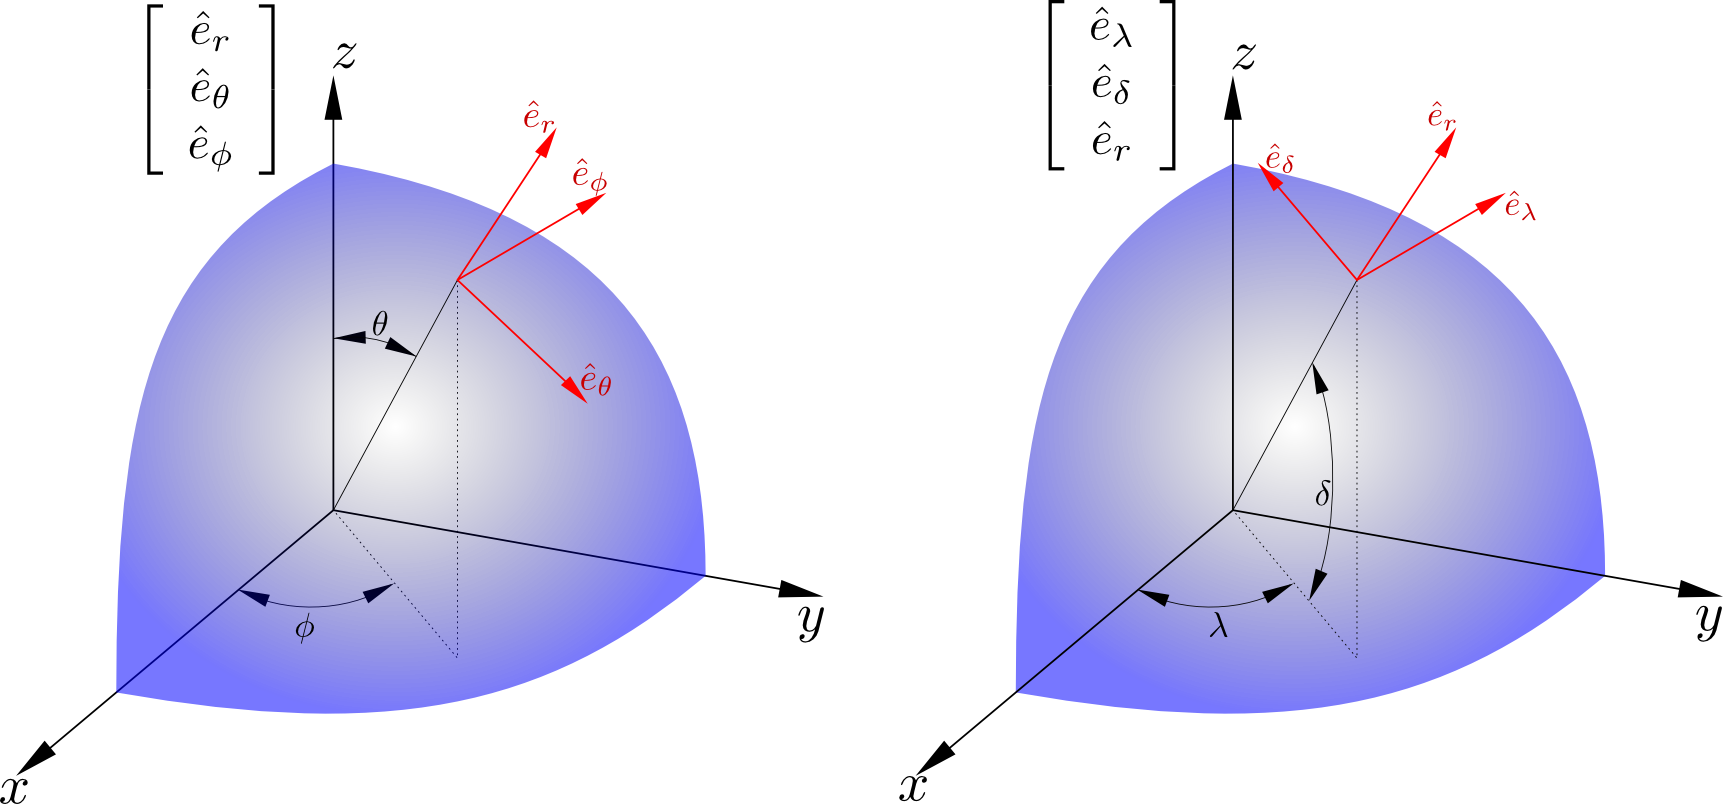
\includegraphics{coordinate_transformations.png}}
  \caption{Polar coordinates. Left: Spherical-polar coordinates where $\phi$ is the azimuthal angle and $\theta$ is the polar angle. Right: Longitude-latitude coordinates where $\lambda$ denotes longitude and $\delta$ denotes latitude.}
  \label{fig:polarCoordinates}
\end{figure}
\par
The transformation routines also feature C-interoperable routines so that the
tansformations can also be called from C/C++ code. The C function prototypes are
located in \lstinline{include/coordinates.h}.
\par
The following lists the availabe transformations:
\begin{itemize}
\item{\textbf{Spherical-polar to Cartesian}}\\
Fortran routine: \lstinline{spherical_polar_2_cartesian}\\
Fortran routine unit-test: \lstinline{femtools/tests/test_spherical_polar_2_cartesian.F90}\\
C-inter-operable wrapper: \lstinline{spherical_polar_2_cartesian_c}\\
C-inter-operable wrapper unit-test: \lstinline{femtools/tests/test_spherical_polar_2_cartesian_c.F90}\\
Interface: describe routine interface, state that angles are expected in radians\\
Short description.

\item{\textbf{Cartesian to Spherical-polar}}\\
Fortran routine: \lstinline{cartesian_2_spherical_polar}\\
Fortran routine unit-test: \lstinline{femtools/tests/test_cartesian_2_spherical_polar.F90}\\
C-inter-operable wrapper: \lstinline{cartesian_2_spherical_polar_c}\\
C-inter-operable wrapper unit-test: \lstinline{femtools/tests/test_cartesian_2_spherical_polar_c.F90}\\
Interface: describe routine interface, state that angles are returned in radians\\
Short description.
\end{itemize}
\par
A python version of the transformation routines is available, contained in the module \lstinline{python/GFD_basisChange_tools.py}. Example of use in \lstinline{tests/data/on_sphere_rotations/construct_fields.py}, where the dataset used in the unit-tests is constructed.



\chapter{State dictionaries}\targetlabel{chap:state}

The state of a system of differential equations is determined by a number of
fields together. State objects provide a mechanism for grouping together
arbitrary collections of fields, meshes, matrices and sparsities which are
in some way related. For many applications, there will be a single state
object which encompasses all of the data in that simulation, however more
complex simulations may require more. For example, a multiphase flow
simulation might have one state object for each fluid phase. The velocity,
pressure, density and other fields belonging to each phase would be listed
in that phase.

\section{Inserting and extracting objects in states}



\section{Aliased fields and listing the same field in multiple state
  dictionaries}\label{sec:alias} 

Because a state dictionary simply holds a reference to a number of fields,
it is perfectly possible to insert the same field in multiple state
dictionaries. In the example of multiphase flow, this might be because there
is a single pressure field applicable to all of the phases. Storing the
same field in the state dictionary for each phase can be a simplyfying step
which also allows for general code which may need to be aware of the
multiphase nature of the simulation.

However, it is often desirable or necessary to have one state dictionary
which is the defined owner of a particular field and which, for example,
might be the only state via which the field is updated. For this purpose it
is possible to designate a field descriptor as being an \emph{alias}\ of the
primary field. To specify that a field descriptor is an alias, set the
\lstinline+aliased+ component of the descriptor to \lstinline+.true.+. For
example:
\begin{lstlisting}
function make_aliased_field(field) result (alias)
  implicit none
  use fields
  type(@\scalarfield@) :: alias 
  type(@\scalarfield@), intent(in) :: field 
  
  alias=field
  alias%aliased=.true.

end function
\end{lstlisting}
This function returns a variable containing the same field as the input, but
the field descriptor is a copy and the \lstinline+aliased+ component has
been set to \lstinline+.true.+. The aliased status of a field can be queried
using the \hyperlink{proc:aliased}{aliased}\ routine. 

\chapter{Reference counting}\targetlabel{chap:refcount}

The key data types described here share complex relationships. For example,
a single mesh might be used by any number of fields in a wide range of
routines in a programme. This presents an immediate challenge for data
management: how does the programme know when it is safe to deallocate the
memory associated with the mesh? Of course that mesh in turn depends on an
element type which must not be deallocated for as long as the mesh exists.

The solution to this problem which is adopted here is the reference
counting. In this system, each data object records the number of other
objects which are currently using it. When a new data object is created, the
reference count associated with each object on which it depends is
increased, and when an object is destroyed, the reference count of each on
which it depends is decreased. When the reference count of an object falls
to zero, the object itself is destroyed and the memory associated with it
freed.

As a brief example, consider just the case of \lstinline+element_type+
objects and the \lstinline+quadrature_type+ objects on which they
depend. Suppose we have the subroutine shown in figure
\ref{fig:refcount}\ which produces two elements. In order to produce the
elements, we first generate a quadadrature object by calling
\lstinline+make_quadrature+. This produces a new quadrature object and sets
it reference count to 1. Next we call \lstinline+make_element_shape+ to
produce the first element object, \lstinline+element1+. Since
\lstinline+element1+ uses quadrature, it increments the reference count of
the quadrature object. \lstinline+quadrature+  now has a reference count of 2
and \lstinline+element1+ has a reference count of 1. We next call
\lstinline+make_element_shape+ again to produce \lstinline+element2+. At this stage
\lstinline+quadrature+ has a reference count of 3: the original reference
created with the object itself plus one each created by \lstinline+element1+
and \lstinline+element2+. Finally, since we have finished using \lstinline+quadrature+
to generate new elements, we call \lstinline+deallocate(quadrature)+. This
destroys the original reference which we created and reduces the reference
count of \lstinline+quadrature+ to 2. However, since the reference count of
\lstinline+quadrature+ is still positive, the object itself is not destroyed
and the memory associated with it is not freed. This is, in fact, the
desired behaviour as the quadrature object must still be available for use
by the elements we created. 

Eventually, when the first element is no longer required, the program will call:
\begin{lstlisting}
  call deallocate(element1)
\end{lstlisting}
Assuming that there are no other objects which are using
\lstinline+element1+, this will reduce the reference count of
\lstinline+element1+ to 0 and it will be destroyed and its memory freed.
This will in turn cause the reference count of the quadrature object to be
reduced to 1. At the point at which \lstinline+element2+ is deallocated, the
reference count of the quadrature will drop to 0 and it will finally be
actually destroyed and its memory freed.

\begin{figure}[ht]
  \begin{lstlisting}
subroutine generate_elements(element1, element2) 
  use quadrature 
  use shape_functions 
  type(element_type), intent(out) :: element1, element2
  type(quadrature_type) :: quadrature

  quadrature=make_quadrature(...)  
  ! The reference count of quadrature is 1.

  element1=make_element_shape(... degree=1, quad=quadrature ...)  
  ! The reference count of quadrature is 2.

  element2=make_element_shape(... degree=2, quad=quadrature ...)  
  ! The reference count of quadrature is 3.

  call deallocate(quadrature) 
  ! The reference count of quadrature is 2.

end subroutine generate_elements
  \end{lstlisting}
  \caption{The reference count of a quadrature object as it is created and used
  to form elements. Finally, one of the references to quadrature is
  discarded by calling deallocate.}
\label{fig:refcount}
\end{figure}

\section{Creating and destroying references}

\subsection{Allocate}

When the \lstinline+allocate+ subroutine is called for an object, this
allocates a new data space for that object and creates a corresponding
reference count for that object, which is set to 1. 

In addition, the reference count of any object which the new object
\emph{directly}\ depends on is increased by 1. For example, when a field is
allocated, the reference count of the \meshtype on which that field is based
on is increased by one. In other words the field \emph{holds a reference}\
to the mesh.

The reference counts of objects which the new field only indirectly depends
on are not affected by a call to allocate. For example, a \meshtype\ holds a
reference to the \elementtype\ on which the mesh is based. When a field is
allocated using that \meshtype\ object, the reference count of the
corresponding \elementtype\ is unchanged. 

It is important to note that these remarks apply only to the \allocate\
subroutine called on a reference-counted object. The Fortran \allocate\
statement has no effect on reference counts.

\subsection{Deallocate}\label{sec:deallocate}

When \lstinline+deallocate+ is called for an object, the reference count of
that object is decreased by 1. If, after this operation, the reference count
is still positive, \lstinline+deallocate+ returns immediately and the object
remains allocated. On the other hand, if the reference count has fallen to 0
then the data space associated with the object is deallocated thereby
destroying the object.

In other words, routines call \lstinline+deallocate+ in order to release a
reference which they hold. The object itself is only destroyed once there
are no more references to it held. 

For objects which hold references to other objects, for example a field
holds a reference to the \meshtype\ on which it is based, the reference to
the other object is released when the first object is destroyed. If this
causes the reference count on the other object to fall to 0, then this will
result in the deallocation of the other object too. Naturally this in turn
may cause further references to be released and any unused objects to be
destroyed.

Calling \deallocate\ on a state dictionary will cause the dictionary to
delete the reference it holds to each of the objects in the dictionary.

As with \allocate\ only the \deallocate\ routines associated with
reference-counted objects will destroy references. The Fortran \deallocate\
object has no effect on reference counts.


\subsection{Inserting into state}\label{sec:refcount_state}

A state dictionary holds a reference to each object it contains. Inserting
an object into a state therefore increments the reference count of that
object. A direct result of this is that if an object is created and
immediately inserted into a state, the reference count of that object will
be 2. If it is desired that the object should be controlled by that state
dictionary and destroyed when that state dictionary is deallocated, it will
be necessary to call \deallocate\ on the object after it is inserted into
the state in order to reduce its reference count to 1.

\subsection{Extracting from  states}

The usual model of use of objects in a state dictionary is that they are
accessed but remain under the control of the dictionary. For example, a
number of the fields in a state may be extracted and updated each timestep
but the fields remain in the state at the end of the timestep. 

To make this morel of use as natural as possible, extracting an object from
a state dictionary does not increase the reference count of that
object. Rather, it could be thought that the reference is borrowed from the
state but still belongs to the state. This means that a routine which
extracts an object from a state should not deallocate that object when it is
finished with it. To do so would invalidly destroy the reference held by the
state.

A consequence of this model is that if the state dictionary is itself deallocated
before the extracting routine has finished with the object, the object may
be destroyed and the pointer made invalid. Should it be necessary to
preserve a reference to an object during the deallocation of the state
object or after control passes from the routine extracting the object, this
can be achieved by calling \lstinline+incref+\ on the object. In this case,
it will be necesary to deallocate the object in order to destroy this
reference and avoid a memory leak.

\subsection{Incref}

In some circumstances, it may be necessary to manually create a new
reference to an object. The usual example would be where an object is
extracted from a state dictionary and the extracting routine wishes to
ensure that that object is not destroyed when control passes to another
routine. The subroutine \lstinline+incref+\ is provided for this purpose. Calling
\lstinline+incref+\ on an object increases the reference count of that
object by 1. It is essential that code which manually increments references
ensures that those references are destroyed by an appropriate \deallocate
call. Failure to do so is likely to result in a memory leak.


\section{Creating new reference counted data types}


\section{Memory accounting diagnostics}

\begin{table}[t]
  \centering
  \begin{tabular}{p{10em}lp{.5\textwidth}}
    \textbf{Data structure} &\textbf{Accounting bin} &\textbf{Information
      recorded}\\\hline\hline
    \meshtype & MeshMemory & element-node, face-node and face-element
    lists. Boundary ID and surface node lists. \\
    & MatrixSparsityMemory & element-element map.\\
    & MatrixMemory & element-face map.\\\hline
    \scalarfield & ScalarFieldMemory & nodal coefficient
    values.\\\hline
    \vectorfield & VectorFieldMemory & nodal coefficient
    values.\\\hline
    \tensorfield & TensorFieldMemory & nodal coefficient values.\\\hline
    csr\_sparsity & MatrixSparsityMemory & matrix nonzero locations.\\\hline
    csr\_matrix block\_csr\_matrix & MatrixMemory & matrix
    nonzero values.\\\hline\hline
  \end{tabular}
  \caption{Forms of data about which memory accounting information is
    stored. Note that since the \meshtype\ data structure contains some
    information which is stored as sparse matrices, some mesh data is
    recorded as sparse matrix data.}
  \label{tab:memory}
\end{table}

Femtools  maintains some accounting information concerning the amount of
memory allocated to reference counted objects. This is useful for diagnosing
which data structures occupy the most memory, although it is important to
note that the memory recorded here will not account for the total amount of
memory allocated by a program using the femtools library: only the large
arrays associated with the data objects listed here are stored.

Memory accounting data is recorded under a number of headings: MeshMemory,
ScalarFieldMemory, VectorFieldMemory, TensorFieldMemory,
MatrixSparsityMemory and MatrixMemory. There is also a TotalMemory heading
which records all of the memory for which accounting data is available.
Table \ref{tab:memory}\ shows for each data object, which memory is logged
and under which category. At this stage, not all memory associated with
field boundary conditions and parallel halo data is logged.

For each memory heading, the current memory usage as well as the maximum and
minimum ever used are stored. It is also possible to reset the maximum and
minimum values, in which case the maximum and minumum values constitute the
maximum and minimum values since the last reset. This enables timestepping
simulations to log the minimum and maximum memory usage in each timestep. 

\subsection{Memory statistics in the .stat file}

If the \lstinline+diagnostic_variables+ module is employed to produce a
.stat file then the maximum and minimum values will be reset
after the .stat file entry for each timestep is written. For each memory
heading, the .stat file will contain fields recording the minimum, maximum
and current memory usage.

\part{Procedure reference}


\chapter{General principles for procedures}

Much of Femtools is designed in an essentially object-oriented manner and
many of the procedures in the library should be understood as methods
belonging to the data objects on which they act. In keeping with widespread
practice, the first argument of a method is the data object on which it
acts. This should be followed by any arguments which control which part of
the object is affected. The next arguments are the input data, if any and
finally any status variable.

\section{Field, mesh and matrix interfaces}

Fields, meshes and matrices have a number of common features which makes
many of their methods amenable to consistent interfaces. To the extent to
which it is applicable, methods for these data types should have interfaces
of the following form:
\begin{lstlisting}[language=bnf]
  procedure_name(object[, dims][, items][, values][, stat])
\end{lstlisting}
The items in square brackets ([]) are optional. All of the arguments other
than the object itself may not appear in all interfaces however those which
are present should appear in this order. For example, the version of the
\hyperlink{proc:fieldaddto}{addto}\ routine which sets a single component of
a tensor field at one node has the argument sequence:
\begin{lstlisting}
  addto(field, dim1, dim2, node_number, val)
\end{lstlisting}

\section{Status arguments}

Routines which might not succeed typically have an optional integer output
argument named \stat. If \stat\ is present and the procedure returns
successfully, it is set to zero while if an error occurs it is set to a
procedure-specific non-zero value. If \stat\ is not present and an error
occurs then execution will terminate with an error.


\chapter{Field and mesh methods}\targetlabel{chap:fieldmeshmethods}


\section{Global field and mesh enquiry routines}

These routines return a single value for an entire mesh or field.

\procedure{mesh\_dim}{proc:meshdim}

\begin{lstlisting}
pure function mesh_dim(mesh)
  integer :: mesh_dim
  type(@\meshtype@), intent(in) :: mesh
\end{lstlisting}

\begin{lstlisting}
pure function mesh_dim(field)
  integer :: mesh_dim
  type(@\anyfield@), intent(in) :: field
\end{lstlisting}

Return the topological dimension of the mesh or the mesh associated with the
field provided. Note that in the case of a vector or tensor field, this may
be different from the topological dimension of the mesh may be different
from the dimension of the data in the field.

\procedure{mesh\_periodic}{proc:meshperiodic}

\begin{lstlisting}
pure function mesh_periodic(mesh)
  logical :: mesh_periodic
  type(@\meshtype@), intent(in) :: mesh
\end{lstlisting}

\begin{lstlisting}
pure function mesh_periodic(field)
  logical :: mesh_periodic
  type(@\anyfield@), intent(in) :: field
\end{lstlisting}

Returns true if the mesh or the mesh associated with the field provided is
periodic in any dimension.

\procedure{node\_count}{proc:nodecount}

\begin{lstlisting}
pure function node_count(mesh)
  integer :: node_count
  type(@\meshtype@), intent(in) :: mesh
\end{lstlisting}

\begin{lstlisting}
pure function node_count(field)
  integer :: node_count
  type(@\anyfield@), intent(in) :: field
\end{lstlisting}

Return the number of nodes in the mesh or field provided.

\procedure{element\_count}{proc:elementcount}

\begin{lstlisting}
pure function element_count(mesh)
  integer :: element_count
  type(@\meshtype@), intent(in) :: mesh
\end{lstlisting}

\begin{lstlisting}
pure function element_count(field)
  integer :: element_count
  type(@\anyfield@), intent(in) :: field
\end{lstlisting}

Return the number of elements in the mesh or field provided.

\procedure{surface\_element\_count}{proc:surfaceelementcount}

\begin{lstlisting}
pure function surface_element_count(mesh)
  integer :: surface_element_count
  type(@\meshtype@), intent(in) :: mesh
\end{lstlisting}

\begin{lstlisting}
pure function surface_element_count(field)
  integer :: surface_element_count
  type(@\anyfield@), intent(in) :: field
\end{lstlisting}

Return the number of surface elements in the mesh or field provided.

\procedure{unique\_surface\_element\_count}{proc:uniquesurfaceelementcount}

\begin{lstlisting}
pure function unique_surface_element_count(mesh)
  integer :: unique_surface_element_count
  type(@\meshtype@), intent(in) :: mesh
\end{lstlisting}

\begin{lstlisting}
pure function unique_surface_element_count(field)
  integer :: unique_surface_element_count
  type(@\anyfield@), intent(in) :: field
\end{lstlisting}

Return the number of unique surface elements in the mesh or field provided. When
using internal boundaries, the facets on the internal boundary (which have a
non-zero surface\_id associated with them), are included in the surface mesh.
These interior facets come in pairs corresponding to the two facets associated
with the two adjacent elements on either side of the internal boundary. The
facets of the surface mesh numbered one to
\hyperlink{proc:uniquesurfaceelementcount}{unique\_surface\_element\_count}
loop through all facets, with only one of each pair of internal facets
appearing. The second facet of each pair is numbered with a facet number bigger
than
\hyperlink{proc:uniquesurfaceelementcount}{unique\_surface\_element\_count}
but smaller or equal to
\hyperlink{proc:surfaceelementcount}{surface\_element\_count}. If there are no
internal facets, both counts return the same number. In finite element assembly
code
\hyperlink{proc:uniquesurfaceelementcount}{unique\_surface\_element\_count}
should typically be used, as boundary conditions should be applied on both sides of the
internal boundary, whereas
\hyperlink{proc:uniquesurfaceelementcount}{unique\_surface\_element\_count}
may appear in parts of the code that deal with the geometry of the mesh.


\procedure{face\_count}{proc:facecount}

\begin{lstlisting}
pure function face_count(mesh)
  integer :: face_count
  type(@\meshtype@), intent(in) :: mesh
\end{lstlisting}

\begin{lstlisting}
pure function face_count(field)
  logical :: face_count
  type(@\anyfield@), intent(in) :: field
\end{lstlisting}

Return the number of faces in the mesh or field provided. Note that this
includes all interior faces, not just facets that have a surface\_id
associated with them (for which see
\hyperlink{proc:surfaceelementcount}{surface\_element\_count} above). Note
also that on internal faces, there is a separate face for each of the two
elements adjacent to the face.

\procedure{aliased}{proc:aliased}
\module{state\_module}

\begin{lstlisting}
pure function aliased(field)
  type(@\anyfield@), intent(in) :: field
  logical :: aliased
\end{lstlisting}

Return \lstinline+.true.+ if \lstinline+field+ is an alias. See section
\ref{sec:alias}\ for information on aliased fields.


\section{Element enquiry routines}

These routines return information about the properties of a single element
in a field or mesh.

\procedure{ele\_loc}{proc:eleloc}

\begin{lstlisting}
pure function ele_loc(mesh, ele_number)
  integer :: ele_loc
  type(@\meshtype@), intent(in) :: mesh
  integer, intent(in) :: ele_number
\end{lstlisting}

\begin{lstlisting}
pure function ele_loc(field, ele_number)
  integer :: ele_loc
  type(@\anyfield@), intent(in) :: field
  integer, intent(in) :: ele_number
\end{lstlisting}

Return the number of nodes in element \lstinline+ele_number+ of the field
or mesh provided. Note that in the current implementation, this is always a
constant value for all elements. This is expected to change in the future.

\procedure{ele\_and\_faces\_loc}{proc:elefacesloc}

\begin{lstlisting}
pure function ele_and_faces_loc(mesh, ele_number)
  integer :: ele_and_faces_loc
  type(@\meshtype@), intent(in) :: mesh
  integer, intent(in) :: ele_number
\end{lstlisting}

\begin{lstlisting}
pure function ele_and_faces_loc(field, ele_number)
  integer :: ele_and_faces_loc
  type(@\anyfield@), intent(in) :: field
  integer, intent(in) :: ele_number
\end{lstlisting}

Return the number of nodes in element \lstinline+ele_number+ of the field
or mesh provided plus the number of nodes in each of the adjacent
faces. This is primarily useful for calculating the size of temporary
matrices used in the local assembly of discontinuous Galerkin operators
which include face integrals. Figure \ref{fig:elefacesloc}\ illustrates the
calculation performed by this function for a linear discontinuous triangular
element.

\begin{figure}[ht]
  \centering
  \xfig{cq_stencil}
  \caption{Illustration of the area included in the node count for
    ele\_and\_faces\_loc for a linear triangular element. In this case the
    element has 3 nodes and each of the three neighbouring faces has 2 nodes
    so the return value is 9.}
  \label{fig:elefacesloc}
\end{figure}
Note that in the current implementation, this is always a
constant value for all elements. This is expected to change in the future.

\procedure{ele\_vertices}{proc:elevertices}

\begin{lstlisting}
pure function ele_vertices(mesh, ele_number)
  integer :: ele_vertices
  type(@\meshtype@), intent(in) :: mesh
  integer, intent(in) :: ele_number
\end{lstlisting}

\begin{lstlisting}
pure function ele_vertices(field, ele_number)
  integer :: ele_vertices
  type(@\anyfield@), intent(in) :: field
  integer, intent(in) :: ele_number
\end{lstlisting}

Return the number of vertices in element \lstinline+ele_number+ of the field
or mesh provided. Vertices are a purely geometric concept so a triangle
always has three vertices regardless of the degree of polynomials used as 
basis functions. In contrast, the number of nodes in an element is a
function of the degree of the polynomial basis functions. For example, a
quadratic triangle has six nodes.

Note that in the current implementation, this is always a
constant value for all elements. This is expected to change in the future.


\procedure{ele\_ngi}{proc:elengi}

\begin{lstlisting}
pure function ele_ngi(mesh, ele_number)
  integer :: ele_ngi
  type(@\meshtype@), intent(in) :: mesh
  integer, intent(in) :: ele_number
\end{lstlisting}

\begin{lstlisting}
pure function ele_ngi(field, ele_number)
  integer :: ele_ngi
  type(@\anyfield@), intent(in) :: field
  integer, intent(in) :: ele_number
\end{lstlisting}

Return the number of quadrature points in element \lstinline+ele_number+ of the field
or mesh provided. Note that in the current implementation, this is always a
constant value for all elements. This is expected to change in the future.

\procedure{ele\_nodes}{proc:ele_nodes}

\begin{lstlisting}
function ele_nodes(mesh, ele_number)
  integer, dimension(:), pointer :: ele_nodes
  type(@\meshtype@),intent(in) :: mesh
  integer, intent(in) :: ele_number
\end{lstlisting}

\begin{lstlisting}
function ele_nodes(field, ele_number)
  integer, dimension(:), pointer :: ele_nodes
  type(@\anyfield@),intent(in) :: field
  integer, intent(in) :: ele_number
\end{lstlisting}

Return a pointer to a vector containing the global node numbers of
element \lstinline+ele_number+ in the mesh provided or in the mesh
associated with the field provided. For example, if \lstinline+this_mesh+ is the
mesh shown in figure \ref{fig:meshnumbering}, then
\lstinline+ele_nodes(this_mesh, 5)+ will return a pointer to a 3-vector
containin the node numbers 3, 6 and 7. No guarantees are made about the
order in which these node numbers will be arranged. 

\section{Face enquiry routines}

These routines return information about the properties of a single element face
in a field or mesh.

\procedure{face\_loc}{proc:faceloc}

\begin{lstlisting}
pure function face_loc(mesh, face_number)
  integer :: face_loc
  type(@\meshtype@), intent(in) :: mesh
  integer, intent(in) :: face_number
\end{lstlisting}

\begin{lstlisting}
pure function face_loc(field, face_number)
  integer :: face_loc
  type(@\anyfield@), intent(in) :: field
  integer, intent(in) :: face_number
\end{lstlisting}

Return the number of nodes in face \lstinline+face_number+ of the field
or mesh provided. Note that in the current implementation, this is always a
constant value for all faces. This is expected to change in the future.

\procedure{face\_vertices}{proc:facevertices}

\begin{lstlisting}
pure function face_vertices(mesh, face_number)
  integer :: face_vertices
  type(@\meshtype@), intent(in) :: mesh
  integer, intent(in) :: face_number
\end{lstlisting}

\begin{lstlisting}
pure function face_vertices(field, face_number)
  integer :: face_vertices
  type(@\anyfield@), intent(in) :: field
  integer, intent(in) :: face_number
\end{lstlisting}

Return the number of vertices in face \lstinline+face_number+ of the field
or mesh provided. Vertices are a purely geometric concept so a triangle
always has three vertices regardless of the degree of polynomials used as 
basis functions. In contrast, the number of nodes in an face is a
function of the degree of the polynomial basis functions. For example, a
quadratic triangle has six nodes.

Note that in the current implementation, this is always a
constant value for all faces. This is expected to change in the future.


\procedure{face\_ngi}{proc:facengi}

\begin{lstlisting}
pure function face_ngi(mesh, face_number)
  integer :: face_ngi
  type(@\meshtype@), intent(in) :: mesh
  integer, intent(in) :: face_number
\end{lstlisting}

\begin{lstlisting}
pure function face_ngi(field, face_number)
  integer :: face_ngi
  type(@\anyfield@), intent(in) :: field
  integer, intent(in) :: face_number
\end{lstlisting}

Return the number of quadrature points in face \lstinline+face_number+ of the field
or mesh provided. Note that in the current implementation, this is always a
constant value for all faces. This is expected to change in the future.

\procedure{face\_local\_nodes}{proc:facelocalnodes}

\begin{lstlisting}
function face_local_nodes(mesh, face_number)
  integer, dimension(:), pointer :: face_local_nodes
  type(@\meshtype@),intent(in) :: mesh
  integer, intent(in) :: face_number  
\end{lstlisting}

\begin{lstlisting}
function face_local_nodes(field, face_number)
  integer, dimension(:), pointer :: face_local_nodes
  type(@\anyfield@),intent(in) :: field
  integer, intent(in) :: face_number  
\end{lstlisting}

Return a pointer to a vector containing the \emph{local} node numbers of
face \lstinline+face_number+ in the  mesh provided or in the mesh
associated with the field provided. Note that these are the local numbers in
the element containing face.

\procedure{face\_global\_nodes}{proc:faceglobalnodes}

\begin{lstlisting}
function face_global_nodes(mesh, face_number)
  integer, dimension(:), pointer :: face_global_nodes
  type(@\meshtype@),intent(in) :: mesh
  integer, intent(in) :: face_number  
\end{lstlisting}

\begin{lstlisting}
function face_global_nodes(field, face_number)
  integer, dimension(:), pointer :: face_global_nodes
  type(@\anyfield@),intent(in) :: field
  integer, intent(in) :: face_number  
\end{lstlisting}

Return a pointer to a vector containing the \emph{global} node numbers of
face \lstinline+face_number+ in the  mesh provided or in the mesh
associated with the field provided. 

\section{Data retrieval routines}

\procedure{ele\_val}{proc:eleval}

Return the value of a field at all of the nodes in an element. The precise
shape of the function value depends on the rank and dimension of the field.

\begin{lstlisting}
function ele_val(field, ele_number) 
  type(@\scalarfield@), intent(in) :: field
  integer, intent(in) :: ele_number
  real, dimension(@\eleloc@(field, ele_number)) :: ele_val
\end{lstlisting}
The scalar field version of this routine returns a vector with length equal
to the number of nodes in this element.

\begin{lstlisting}
function ele_val(field, ele_number)
  type(@\vectorfield@),intent(in) :: field
  integer, intent(in) :: ele_number
  real, dimension(field%dim, @\eleloc@(field, ele_number)) :: ele_val
\end{lstlisting}
\begin{lstlisting}
function ele_val(field, ele_number)
  type(@\tensorfield@),intent(in) :: field
  integer, intent(in) :: ele_number
  real, dimension(field%dim, field%dim, @\eleloc@(field, ele_number)) :: ele_val
\end{lstlisting}
Note that for these vector and tensor versions of the routine, the dim
dimensions come first, followed by the number of element nodes.

\begin{lstlisting}
function ele_val(field, ele_number, dim) 
  type(@\vectorfield@), intent(in) :: field
  integer, intent(in) :: ele_number, dim
  real, dimension(@\eleloc@(field, ele_number)) :: ele_val
\end{lstlisting}
\begin{lstlisting}
function ele_val(field, ele_number, dim1, dim2) 
  type(@\tensorfield@), intent(in) :: field
  integer, intent(in) :: ele_number, dim1, dim2
  real, dimension(@\eleloc@(field, ele_number)) :: ele_val
\end{lstlisting}
These versions of the routine return the value of a single component of the
vector or tensor field at all of the nodes of the element. 

\procedure{ele\_val\_at\_quad}{proc:elevalatquad}

\begin{lstlisting}
function ele_val_at_quad_scalar(field, ele_number)
  type(@\scalarfield@),intent(in) :: field
  integer, intent(in) :: ele_number
  real, dimension(@\elengi@(field, ele_number)) :: ele_val_at_quad  
\end{lstlisting}

\procedure{face\_val}{proc:faceval}

Return the value of a field at all of the nodes in an face. The precise
shape of the function value depends on the rank and dimension of the field.

\begin{lstlisting}
function face_val(field, face_number) 
  type(@\scalarfield@), intent(in) :: field
  integer, intent(in) :: face_number
  real, dimension(@\faceloc@(field, face_number)) :: face_val
\end{lstlisting}
The scalar field version of this routine returns a vector with length equal
to the number of nodes in this face.

\begin{lstlisting}
function face_val(field, face_number)
  type(@\vectorfield@),intent(in) :: field
  integer, intent(in) :: face_number
  real, dimension(field%dim, @\faceloc@(field, face_number)) :: face_val
\end{lstlisting}
\begin{lstlisting}
function face_val(field, face_number)
  type(@\tensorfield@),intent(in) :: field
  integer, intent(in) :: face_number
  real, dimension(field%dim, field%dim, @\faceloc@(field, face_number)) :: face_val
\end{lstlisting}
Note that for these vector and tensor versions of the routine, the dim
dimensions come first, followed by the number of face nodes.

\begin{lstlisting}
function face_val(field, face_number, dim) 
  type(@\vectorfield@), intent(in) :: field
  integer, intent(in) :: face_number, dim
  real, dimension(@\faceloc@(field, face_number)) :: face_val
\end{lstlisting}
\begin{lstlisting}
function face_val(field, face_number, dim1, dim2) 
  type(@\tensorfield@), intent(in) :: field
  integer, intent(in) :: face_number, dim1, dim2
  real, dimension(@\faceloc@(field, face_number)) :: face_val
\end{lstlisting}
These versions of the routine return the value of a single component of the
vector or tensor field at all of the nodes of the face. 

\procedure{node\_val}{proc:nodeval}

Return the value of a field at one or more specified nodes. The shape of the
value returned is given by the rank and dimension of the field and the
number of nodes queried.

\begin{lstlisting}
function node_val(field, node_number)
  type(@\scalarfield@),intent(in) :: field
  integer, intent(in) :: node_number
  real :: node_val
\end{lstlisting}
\begin{lstlisting}
function node_val(field, node_numbers)
  type(@\scalarfield@),intent(in) :: field
  integer, dimension(:), intent(in) :: node_numbers
  real, dimension(size(node_numbers)) :: node_val
\end{lstlisting}

For a scalar field, there is clearly one real number per node.

\begin{lstlisting}
function node_val(field, node_number)
  type(@\vectorfield@),intent(in) :: field
  integer, intent(in) :: node_number
  real, dimension(field%dim) :: node_val
\end{lstlisting}
\begin{lstlisting}
function node_val(field, node_numbers)
  type(@\vectorfield@),intent(in) :: field
  integer, dimension(:), intent(in) :: node_numbers
  real, dimension(field%dim, size(node_numbers)) :: node_val
\end{lstlisting}
\begin{lstlisting}
function node_val(field, node_number)
  type(@\tensorfield@),intent(in) :: field
  integer, intent(in) :: node_number
  real, dimension(field%dim, field%dim) :: node_val
\end{lstlisting}
\begin{lstlisting}
function node_val(field, node_numbers)
  type(@\tensorfield@),intent(in) :: field
  integer, dimension(:), intent(in) :: node_numbers
  real, dimension(field%dim, field%dim, size(node_numbers)) :: node_val
\end{lstlisting}
In the result of the full vector and tensor versions of this routine, the
dimension components come first followed by the number of nodes, for the
multiple node version.

\begin{lstlisting}
function node_val(field, node_number, dim)
  type(@\vectorfield@),intent(in) :: field
  integer, intent(in) :: node_number
  integer, intent(in) :: dim
  real :: node_val
\end{lstlisting}
\begin{lstlisting}
function node_val(field, node_numbers, dim)
  type(@\vectorfield@),intent(in) :: field
  integer, dimension(:), intent(in) :: node_numbers
  integer, intent(in) :: dim
  real, dimension(size(node_numbers)) :: node_val
\end{lstlisting}
\begin{lstlisting}
function node_val(field, dim1, dim2, node_number)
  type(@\tensorfield@),intent(in) :: field
  integer, intent(in) :: node_number
  integer, intent(in) :: dim1, dim2
  real :: node_val
\end{lstlisting}
\begin{lstlisting}
function node_val(field, dim1, dim2, node_numbers)
  type(@\tensorfield@),intent(in) :: field
  integer, dimension(:), intent(in) :: node_numbers
  integer, intent(in) :: dim1, dim2
  real, dimension(size(node_numbers)) :: node_val
\end{lstlisting}
These versions of the the routine return the value of a single component of
the field at one or more nodes.

\section{Data setting routines}

The routines in this section are typically the field versions of interfaces
which are also available for structures such as sparse matrices.

\procedure{addto}{proc:fieldaddto}

\subsubsection{Adding to node values}

Addto is the generic calling name for a number of subroutines which update
their first argument by adding values to it. The first basic form of this
routine adds a value to one or more nodes of a field. Its generic forms are:

\begin{lstlisting}
subroutine addto(field, node_number, val)
  type(@\anyfield@), intent(inout) :: field
  integer, intent(in) :: node_number
  real, dimension(@\valshape@), intent(in) :: val
\end{lstlisting}
\begin{lstlisting}
subroutine addto(field, node_numbers, val)
  type(@\anyfield@), intent(inout) :: field
  integer, dimension(:), intent(in) :: node_numbers
  real, dimension(@\valshape@, size(nodenumbers)), intent(in) :: val
\end{lstlisting}

The shape of the val argument varies according to the field type:

\begin{tabular}{ll}
  \textbf{field type}& \textbf{\valshape}\\
  \scalarfield & \\
  \vectorfield & \lstinline+field%dim+ \\
  \tensorfield & \lstinline+field%dim, field%dim+
\end{tabular}

In the case of a scalar field, the value is clearly a scalar and so
\valshape\ does not contribute to the rank of \lstinline+val+ at all.

There are related forms of the routine which add to the value of a single
component of a vector or tensor field at one or more nodes:

\begin{lstlisting}
subroutine addto(field, dim, node_number, val)
  type(@\vectorfield@), intent(inout) :: field
  integer, intent(in) :: dim
  integer, intent(in) :: node_number
  real, intent(in) :: val
\end{lstlisting}
\begin{lstlisting}
subroutine addto(field, dim, node_numbers, val)
  type(@\vectorfield@), intent(inout) :: field
  integer, intent(in) :: dim
  integer, dimension(:), intent(in) :: node_numbers
  real, dimension(size(nodenumbers)), intent(in) :: val
\end{lstlisting}
\begin{lstlisting}
subroutine addto(field, dim1, dim2, node_number, val)
  type(@\vectorfield@), intent(inout) :: field
  integer, intent(in) :: dim1, dim2
  integer, intent(in) :: node_number
  real, intent(in) :: val
\end{lstlisting}
\begin{lstlisting}
subroutine addto(field, dim1, dim2, node_numbers, val)
  type(@\vectorfield@), intent(inout) :: field
  integer, intent(in) :: dim1, dim2
  integer, dimension(:), intent(in) :: node_numbers
  real, dimension(size(nodenumbers)), intent(in) :: val
\end{lstlisting}

\subsubsection{Adding fields to each other}

Simple whole field addition operations are only mathematically defined where all of the
fields share the same mesh. Where this is not the case, addto will call
\remapfield\ on field2 to produce a well-defined operation. 

\begin{lstlisting}
subroutine addto(field1, field2, scale)
  type(@\anyfield@), intent(inout) :: field1
  type(@\anyfield@), intent(in) :: field2
  real, intent(in), optional :: scale
\end{lstlisting}

This form of the routine performs the assignment:
\begin{equation}
  F_1(\x) = s \times F_2(\x)
\end{equation}
Clearly the two fields must have the same rank. If scale is not present then
a value of 1.0 is assumed. 

There are also versions of this subroutine which add a scalar field to a
single component of a vector or tensor field:
\begin{lstlisting}
subroutine addto(field1, dim, field2, scale)
  type(@\vectorfield@), intent(inout) :: field1
  integer, intent(in) :: dim
  type(@\scalarfield@), intent(in) :: field2
  real, intent(in), optional :: scale
\end{lstlisting}
\begin{lstlisting}
subroutine addto(field1, dim1, dim2, field2, scale)
  type(@\tensorfield@), intent(inout) :: field1
  integer, intent(in) :: dim1, dim2
  type(@\scalarfield@), intent(in) :: field2
  real, intent(in), optional :: scale
\end{lstlisting}

\procedure{scale}{proc:fieldscale}

The scale family of routines perform various versions of the operation:
\begin{equation}
  F(\x) = s \times F(\x)
\end{equation}
In the simplest version, the input field is simply scaled by a constant
scalar:
\begin{lstlisting}
subroutine scale(field, factor)
  type(@\anyfield@), intent(inout) :: field
  real, intent(in) :: factor
\end{lstlisting}
It is also possible to scale any field by the entries of a scalar field on
the same mesh:
\begin{lstlisting}
subroutine scale(field, sfield)
  type(@\anyfield@), intent(inout) :: field
  type(@\scalarfield@), intent(in) :: sfield
\end{lstlisting}
However, care must be taken in using this routine since the product of the
nodal values is not in general equal to the product of the discretised
fields. Taking the example of two scalar fields $F$ and $G$, this is because:
\begin{equation}
  F(\x)G(\x)\equiv\sum_{\alpha=1}^{\Ndof}\sum_{\beta=1}^{\Ndof}
  f_\alpha\phi_\alpha g_\beta\phi_\beta
  \neq\sum_{\alpha=1}^{\Ndof}f_\alpha g_\alpha\phi_\alpha
\end{equation}
Using the scale subroutine to multiply two fields amounts to the rightmost
expression. Subject to the same caveat, it is also possible to scale a
vector field by another vector field:
\begin{lstlisting}
subroutine scale(field, vfield)
  type(@\anyfield@), intent(inout) :: field
  type(@\vectorfield@), intent(in) :: vfield  
\end{lstlisting}

\procedure{set}{proc:fieldset}

As with \hyperlink{proc:addto}{addto}, set is a family of routines which set
the value of part or all of their first argument.

\subsubsection{Setting node values}

The first version of this routine sets the value of field at one or more
nodes:

\begin{lstlisting}
subroutine set(field, node_number, val) 
  type(@\anyfield@), intent(inout) :: field 
  integer, intent(in) :: node_number
  real, dimension(@\valshape@), intent(in) :: val
\end{lstlisting}
\begin{lstlisting}
subroutine set(field, node_number, val) 
  type(@\anyfield@), intent(inout) :: field 
  integer, dimension(:), intent(in) :: node_number
  real, dimension(@\valshape@, size(nodenumbers)), intent(in) :: val
\end{lstlisting}

The shape of the val argument varies according to the field type:

\begin{tabular}{ll}
  \textbf{field type}& \textbf{\valshape}\\
  \scalarfield & \\
  \vectorfield & \lstinline+field%dim+ \\
  \tensorfield & \lstinline+field%dim, field%dim+
\end{tabular}

In the case of a scalar field, the value is clearly a scalar and so
\valshape\ does not contribute to the rank of \lstinline+val+ at all.

\subsubsection{Setting the whole field to a constant value}

It is sometimes useful to set an entire field to a constant value. This is a
chieved with:
\begin{lstlisting}
subroutine set(field, val)
  type(@\anyfield@), intent(inout) :: field 
  real, dimension(@\valshape@), intent(in) :: val
\end{lstlisting}

Where \valshape\ has the meaning given above. 

\subsubsection{Setting a field to the value of another field}

Setting one field to the value of another field is currently only supported
where the two fields are on the same mesh. 
\begin{lstlisting}
subroutine set(out_field, in_field )
  type(@\anyfield@), intent(inout) :: out_field
  type(@\anyfield@), intent(in) :: in_field
\end{lstlisting}
Clearly for this to be defined, in\_field and out\_field must have the same
rank and dimension. Note that this does not allocate out\_field, so it must
already be allocated.

A related case which occurs frequently when implementing schemes for
time-varying PDEs is that of assigning a linear combination of two other
fields to a field. That is:
\begin{equation}
  F(\x)=\theta F_{\textrm{new}}(\x) + (1-\theta) F_{\textrm{old}}(\x)
\end{equation}
This is achieved with the following form of set:
\begin{lstlisting}
subroutine set(out_field, in_field_new, in_field_old, theta)
  type(@\anyfield@), intent(inout) :: out_field
  type(@\anyfield@), intent(in) :: in_field_new, in_field_old
  real, intent(in) :: theta
\end{lstlisting}

\procedure{zero}{proc:fieldzero}

\begin{lstlisting} 
subroutine zero(field)
  type(@\anyfield@), intent(inout) :: field
\end{lstlisting}

This routine simply sets every entry in field to zero. There are also forms
of this subroutine which zero single vector and tensor field components:

\begin{lstlisting}
subroutine zero(field, dim)
  type(@\vectorfield@), intent(inout) :: field
  integer, intent(in) :: dim
\end{lstlisting}
\begin{lstlisting}
subroutine zero(field, dim1, dim2)
  type(@\tensorfield@), intent(inout) :: field
  integer, intent(in) :: dim1, dim2
\end{lstlisting}


\chapter{State dictionary methods}

State objects provide a unified way of grouping a diverse range of femtools
objects. The list of objects which can be contained in a state dictionary
are listed in table \ref{tab:stateobjects}

\begin{table}[ht]
  \centering
\begin{tabular}{lp{.5\textwidth}}
  \textbf{object} & \textbf{object\_type} \\\hline\hline
  \lstinline+field+ & \anyfield \\
  \lstinline+mesh+ & \meshtype \\
  \lstinline+halo+ & \lstinline+halo_type+ \\
  \lstinline+matrix+ & \lstinline+csr_matrix+\newline 
  \lstinline+block_csr_matrix+\newline
  \lstinline+petsc_csr_matrix+
\end{tabular}
  \caption{List of object argument names and corresponding object types
    supported by the \lstinline+state_type+ and its various access methods.}
  \label{tab:stateobjects}
\end{table}

\section{Inserting objects in states}

\procedure{insert}{proc:stateinsert}
\module{state\_module}

\begin{lstlisting}
subroutine insert(state, @\emph{object}@, name)
  type(state_type), intent(inout) :: state
  type(@\emph{object\_type}@), intent(in) :: @\emph{object}@
  character(len=*), intent(in) :: name
\end{lstlisting}

\begin{lstlisting}
subroutine insert(state, @\emph{object}@, name)
  type(state_type), dimension(:), intent(inout) :: state
  type(@\emph{object\_type}@), intent(in) :: @\emph{object}@
  character(len=*), intent(in) :: name
\end{lstlisting}

These routines insert an object into a state dictionary. The first form
inserts an object into a single state dictionary while the second form
inserts the object into the first state and an alias of the object into each
subsequent state. The \emph{object}\ argument can be any of those listed in
table \ref{tab:stateobjects}.


\section{Extracting objects from states}

Objects in states may be accessed by name or by index. The index of an
object in a state is arbitrary and may change as objects are added to and
deleted from the state so this latter option is mostly of use for iterating
over all of the objects of a particular type in the state. 

In each case, the routine returns a pointer to the object concerned. If the
object is only to be read or if changes are only to be made to the data
space then the pointer may be assigned to a non-pointer variable. On the
other hand, if changes are made to the object descriptor then these should be
made via the pointer in order to ensure that it is the descriptor in the
state dictionary which is updated rather than a local copy.

\subsection{Extracting objects by name}
  
\begin{lstlisting}
function extract_@\emph{object\_type}@(state, name, stat[, allocated])
  type{@\emph{object\_type}@}, pointer :: extract_@\emph{object\_type}@ 
  type(state_type), intent(in) :: state
  character(len=*), intent(in) :: name
  integer, intent(out), optional :: state
  logical, intent(out), optional :: allocated
\end{lstlisting}

\begin{lstlisting}
function extract_@\emph{object\_type}@(state, name, stat[, allocated])
  type{@\emph{object\_type}@}, pointer :: extract_@\emph{object\_type}@ 
  type(state_type), dimension(:), intent(in) :: state
  character(len=*), intent(in) :: name
  integer, intent(out), optional :: state
  logical, intent(out), optional :: allocated
\end{lstlisting}

In each case, the \emph{object\_type}\ can be any of the types listed in
table \ref{tab:stateobjects}. 

The first form of the routine takes a single state dictionary as an
argument. If there is an object of the corresponding type with name matching
\lstinline+name+ then a pointer to that object is returned. If
\stat\ is present then it is set to 0.

If there is no matching object with the correct name in the dictionary then
if \stat\ is present it is set to 1 and the function returns a pointer to a
dummy object whose components should not be accessed. If \stat\ is not
present then execution will halt with an error.

The second form of the routine takes a vector of states and will return the
first object it finds in any of the states matching the name provided. The
return values of the \stat\ argument and the handling of the case where
there is no match is as before.

\subsubsection{Reference counts of objects extracted from states}

With the exception of the extraction of a scalar component from a vector
field discussed below, the extraction of a pointer to an object from a state
does not create a new reference to that object. Consequently the object
returned should not be deallocated as this would result in the premature
destruction of that object. See section \ref{sec:refcount_state}\ for a full
discussion of the interaction between reference counts and state objects.


\subsubsection{Extracting scalar components of vector fields}

It is also possible to extract a single component of a vector field stored
in a state dictionary. The syntax for this is to call
\lstinline+extract_scalar_field+ and provide a logical variable in as the
\lstinline+allocated+ argument. The name of the field should be specified as
\emph{name}\%\emph{n}\ where \emph{name}\ is the name under which the vector
field is stored in the state and \emph{n}\ is the number of the component to
be extracted. If the name and component number match then a new scalar field
descriptor will be allocated and the corresponding data spaces will be
associated with the correct component of the vector.

This form of \lstinline+extract_scalar_field+ extract scalar field can be an
exception to the rule that extracting an object reference from a state
dictionary does not create a new reference. If the \lstinline+allocated+
argument returns \lstinline+.true.+ then a new reference has been created
and the resulting field will need to be deallocated in order for that
reference to be destroyed. 

It is possible to pass a vector of state dictionaries to
\lstinline+extract_scalar_field+ in which case the scalar field returned
will be extracted from the first matching vector field.

\subsection{Extracting objects by index}

It is frequently convenient to perform some action for each object of a
particular type in a state. To facilitate this, the following alternative
form of the extraction routines is provided:

\begin{lstlisting}
function extract_@\emph{object\_type}@(state, index)
  type{@\emph{object\_type}@}, pointer :: extract_@\emph{object\_type}@ 
  type(state_type), intent(in) :: state
  integer, intent(in) :: index
\end{lstlisting}

This routine is available for any of the types in table
\ref{tab:stateobjects}. In each case \lstinline+index+ must not exceed the
number of objects of that type in \lstinline+state+. See 
\hyperlink{proc:objectcounts}{object counts}.


\section{Auxiliary state routines}

\procedure{deallocate}{proc:deallocatestate}

\begin{lstlisting}
subroutine deallocate_state(state)
  type(state_type), intent(inout) :: state
\end{lstlisting}

This routine removes all of the objects from \lstinline+state+ and calls
\deallocate on each of them to release the reference held by the state
object.

\procedure{remove object}{proc:removeobject}

\begin{lstlisting}
subroutine remove_@\emph{object\_type}@(state, name, stat)
  type(state_type), intent(inout) :: state
  character(len=*), intent(in) :: name
  integer, optional, intent(out) :: stat
\end{lstlisting}

If there is an object of the specified type in \lstinline+state+ stored
under the name \lstinline+name+, then that object is removed fron
\lstinline+state+ and \deallocate is called for the object to release the
reference which \lstinline+state+ is holding to it.

If \stat is present then it will be set to 0 for success and nonzero for
failure, which occurs if there was no matching object to remove. If the
routine fails to remove an object and \stat has not been specified,
execution will cease with an error. 

\procedure{object counts}{proc:objectcounts}

\begin{lstlisting}
pure function @\emph{object\_type}@_count(state)
  integer :: @\emph{object\_type}@_count
  type(state_type), intent(in) :: state
\end{lstlisting}

This routine returns the number of objects of the given type stored in the
\lstinline+state+. \emph{object\_type}\ can be any of the types listed in
table \ref{tab:stateobjects}.

\chapter{Element methods}

\section{Quadrature methods}

\procedure{make\_quadrature}{proc:makequadrature}
\module{quadrature}

\begin{lstlisting}
function make_quadrature(vertices, dim, degree, ngi, family, stat)
  type(quadrature_type) :: make_quadrature
  integer, intent(in) :: vertices, dim
  integer, intent(in), optional :: degree, ngi
  integer, intent(in), optional :: family
  integer, intent(out), optional :: stat  
\end{lstlisting}

This routine creates a new \quadraturetype\ object. The element geometry for
which the quadrature is produced is specified by the \lstinline+vertices+
and \lstinline+dim+ arguments. Valid combinations of these are:

\begin{center}
  \begin{tabular}{ccl}
    \textbf{vertices} & \textbf{dim} & \textbf{Element geometry}\\\hline
    1 & 1 & point\\
    2 & 1 & interval\\
    3 & 2 & triangle\\
    4 & 2 & quad\\
    4 & 3 & tet\\
    8 & 3 & hex
  \end{tabular}
\end{center}

The accuracy of the quadrature rule is given by the \lstinline+degree+
argument which specifies the degree of polynomial which will be integrated
exactly by this quadrature rule. If the specified quadrature degree is
unavailable but a higher degree rule is supported then this will be
substituted. Specifying a higher degree than is supported is an error.
An alternative method of specifying the quadrature rule is to directly
specify the number of quadrature points via the \lstinline+ngi+
argument. This approach is deprecated. 

The \lstinline+family+ argument specifies the family of quadrature rules
which should be applied. The default is \lstinline+FAMILY_COOLS+ and this is
the only supported choice for quadrilateral and hexahedral elements. The
available options are:

\begin{center}
  \begin{tabular}{llc}
    \textbf{family}&\textbf{valid geometries} & \textbf{maximum degree}\\\hline
    \lstinline+FAMILY_COOLS+& all & 8 \\
    \lstinline+FAMILY_WANDZURA+& triangle & 30 \\
    \lstinline+FAMILY_GM+& interval,triangle,simplex & 30
  \end{tabular}
\end{center}

If present, \lstinline+stat+ is set to 0 to indicate successful
completion. Errors are indicated by the following values:

\begin{center}
  \begin{tabular}{ll}
    \textbf{stat value} & \textbf{meaning}\\\hline
    \lstinline+QUADRATURE_VERTEX_ERROR+ & Unsupported vertex count.\\
    \lstinline+QUADRATURE_DEGREE_ERROR+ &Quadrature degree requested is not available.\\
    \lstinline+QUADRATURE_DIMENSION_ERROR+ & Elements with this number of dimensions are not available.\\
    \lstinline+QUADRATURE_NGI_ERROR+ & Unsupported number of quadrature points.\\ 
    \lstinline+QUADRATURE_ARGUMENT_ERROR+ & Not enough arguments specified.\\
  \end{tabular}
\end{center}

If the \lstinline+stat+ argument is not present then any error will cause
execution to cease with an error message.

\procedure{deallocate}{proc:deallocatequadrature}
\module{quadrature}

\begin{lstlisting}
subroutine deallocate(quad,stat)
  type(quadrature_type), intent(inout) :: quad
  integer, intent(out), optional :: stat
\end{lstlisting}

This routine releases one reference to \lstinline+quad+. For a full
discussion of deallocation of reference-counted data types see section
\ref{sec:deallocate}.

\section{Shape function methods}

\procedure{make\_element\_shape}{proc:makeelementshape}
\module{shape\_functions}

There are two forms of the \lstinline+make_element_shape+ function. The
first is the basic form:

\begin{lstlisting}
function make_element_shape(vertices, dim, degree, quad, type,&
       stat, quad_s)  
  type(element_type) :: make_element_shape
  integer, intent(in) :: vertices, dim, degree
  type(quadrature_type), intent(in), target :: quad
  integer, intent(in), optional :: type
  integer, intent(out), optional :: stat
  type(quadrature_type), intent(in), optional, target :: quad_s
\end{lstlisting}

This routine formulates a basis for a discrete function space over a single
element. The geometry of the element is defined by the arguments
\lstinline+vertices+ and \lstinline+dim+ as follows:
\begin{center}
  \begin{tabular}{ccl}
    \textbf{vertices} & \textbf{dim} & \textbf{Element geometry}\\\hline
    1 & 1 & point\\
    2 & 1 & interval\\
    3 & 2 & triangle\\
    4 & 2 & quad\\
    4 & 3 & tet\\
    8 & 3 & hex
  \end{tabular}
\end{center}

The integration rule is provided by the \quadraturetype\ argument,
\lstinline+quad+. The geometry of \lstinline+quad+ must match that specified
in this call. 

The argument \lstinline+type+ selects the element family from which the shape
functions should be drawn:

\begin{center}
  \begin{tabular}{ll}
    \textbf{element type} & \textbf{description} \\\hline
    \lstinline+ELEMENT_LAGRANGIAN+ & Equispaced Lagrangian elements.\\
    \lstinline+ELEMENT_LAGRANGIAN+ & $\mathrm{P}1_{\mathrm{NC}}$
    non-conforming elements on triangles.\\
    \lstinline+ELEMENT_CONTROLVOLUME_SURFACE+ & A control
    volume surface interior to the domain.\\
    \lstinline+ELEMENT_CONTROLVOLUMEBDY_SURFACE+ & A control volume surface
    on the boundary of the domain.
  \end{tabular}
\end{center}

\lstinline+ELEMENT_LAGRANGIAN+ is the default.

As with other routines, the \lstinline+stat+ argument, if present, returns 0
for successful completion and a non-zero value otherwise. If
\lstinline+stat+ is not present then unsuccessful completion of the routine
results in the termination of execution and an error message.

The \lstinline+quad_s+ argument provides a mechanism for providing
quadrature for the surfaces of the element. \textbf{Not sure when this is
  used}.

The second form of \lstinline+make_element_shape+ allows an \elementtype\
to be based on another variable of the same type:

\begin{lstlisting}
function make_element_shape(model, vertices, dim, degree, quad, type,&
       stat, quad_s)  
  type(element_type) :: make_element_shape
  type(element_type), intent(in) :: model
  integer, intent(in), optional :: vertices, dim, degree
  type(quadrature_type), intent(in), optional, target :: quad
  integer, intent(in), optional :: type
  integer, intent(out), optional :: stat
  type(quadrature_type), intent(in), optional, target :: quad_s
\end{lstlisting}

In this form of the subroutine, all the arguments are optional except for
\lstinline+model+. Where any argument is absent, the corresponding value
will be taken from \lstinline+model+.

\procedure{deallocate}{proc:deallocateelement}

\begin{lstlisting}
subroutine deallocate(element, stat)
  type(element_type), intent(inout) :: element
  integer, intent(out), optional :: stat
\end{lstlisting}

This routine releases one reference to \lstinline+element+. If this reduces
the reference count to zero, \lstinline+element+ is deallocated and the
quadrature reference held by \lstinline+element+ will be released.

\procedure{local\_coords}{proc:elementlocalcoords}

\begin{lstlisting}
function element_local_coords(n, element)
  integer, intent(in) :: n
  type(element_type), intent(in) :: element    
  real, dimension(local_coord_count(element)) :: element_local_coords
\end{lstlisting}

This routine returns the local coordinates in \lstinline+element+ of the
node with local number \lstinline+n+.

\procedure{local\_coord\_count}{proc:elementlocalcoordcount}

\begin{lstlisting}
function element_local_coord_count(element) 
  integer :: element_local_coord_count
  type(element_type), intent(in) :: element    
\end{lstlisting}

This routine returns the number of local coordinates associated with
\lstinline+element+. The results of the function are as follows:
\begin{center}
  \begin{tabular}{lc}
    \textbf{element geometry} & \textbf{number of local coordinates}\\\hline
    point & 1 \\
    interval & 2 \\
    triangle & 3 \\
    quadrilateral & 2 \\
    tet & 4 \\
    hex & 3
  \end{tabular}
\end{center}

\procedure{eval\_shape}{proc:elementevalshape}

\begin{lstlisting}
pure function eval_shape(shape, node, l)
    real :: eval_shape
    integer, intent(in) :: node
    type(element_type), intent(in) :: shape
    real, dimension(element_local_coord_count(element)), intent(in) :: l
\end{lstlisting}

\begin{lstlisting}
pure function eval_shape(shape, l) result(eval_shape)
  type(element_type), intent(in) :: shape
  real, dimension(element_local_coord_count(element)), intent(in) :: l
  real, dimension(shape%loc) :: eval_shape
\end{lstlisting}

This routine evaluates one or more of the shape functions associated with
the element \lstinline+shape+ at the local coordinates specified by
\lstinline+l+. In the first form of the routine,  \lstinline+node+ is the
local number of the node associated with the shape function to be
evaluated. In the second form, all of the shape functions associated with
the element are evaluated and the results returned as a vector.


\chapter{Functions implementing integrals over elements}

\section{Bilinear forms}

The routines in this section form the local contributions pertaining to a
bilinear form evaluated over a single element. As such they are the building
blocks for the assembly of equations. Many of the arguments are essentially
common across the routines. These are shown in table \ref{tab:form_arguments}.

\begin{table}[ht]
\begin{tabular}{p{5em}ccp{.3\textwidth}}
  \textbf{Argument}&\textbf{Shape}&\textbf{Mathematical notation}&\textbf{Meaning}\\\hline\hline
  \lstinline+shape1+&& $\left\{\phi_i:\ i=1\ldots\Nloc(\phi)\right\}$&The set
  of local basis functions for the \emph{test}\ space on the current
  element.\\\hline 
  \lstinline+shape2+&& $\left\{\hat{\phi}_j:\
    j=1\ldots\Nloc(\hat{\phi})\right\}$&The set of local basis functions for
  the \emph{trial}\ space on the current element.\\\hline 
  \lstinline+dshape1+&$\Nloc\times\Nquad\times\Ndim$&$\left\{\grad\phi_i:\ i=1\ldots\Nloc(\phi)\right\}$&
  The set of gradients of the local basis functions for the \emph{test}\ space on
  the current element.\\\hline
  \lstinline+dshape2+&$\Nloc\times\Nquad\times\Ndim$&$\left\{\grad\hat\phi_j:\ j=1\ldots\Nloc(\hat\phi)\right\}$&
  The set of gradients of the local basis functions for the \emph{trial}\ space on
  the current element.\\\hline
  \lstinline+detwei+&$\Nquad$&$\left\{w_{gi}\left|J^{-1}_{gi}\right|:\
    gi=1\ldots\Nquad\right\}$& 
  The quadrature weights transformed by the change of coordinates from the
  current element to the reference element.\\\hline
  \lstinline+vector+\newline
  \lstinline+vector1+\newline
  \lstinline+vector2+&$\Ndim\times\Nquad$& $\{\v_\alpha:\ \alpha=1\ldots\Ndim(\v)\}$ & A vector
  quantity evaluated at each quadrature point. This might be a value
  returned by \elevalatquad.\\\hline
  \lstinline+tensor+&$\Ndim\times\Ndim\times\Nquad$& $\{\tensor{\tau}_{\alpha\beta}:\
  \alpha,\beta=1\ldots\Ndim(\tensor{\tau})\}$ & A tensor
  quantity evaluated at each quadrature point. This might be a value
  returned by \elevalatquad.
\end{tabular}
  \caption{Common arguments used in linear and bilinear form routines.}\hypertarget{tab:form_arguments}{}\label{tab:form_arguments}
\end{table}

\procedure{shape\_shape}{proc:shapeshape}
\module{fetools}

\begin{lstlisting}
function shape_shape(shape1, shape2, detwei)
  type(element_type), intent(in) :: shape1, shape2
  real, dimension(shape1%ngi), intent(in) :: detwei

  real, dimension(shape1%loc,shape2%loc) :: shape_shape
\end{lstlisting}

This routine constructs the following matrix:
\begin{equation}
  \mat{M}(i,j)=\int_E \phi_{i}\hat{\phi}_{j}\d V\quad
  i=1\ldots\Nloc(\phi),\quad j=1\ldots\Nloc(\hat{\phi}) 
\end{equation}
Where the arguments are as given in table \ref{tab:form_arguments}.

\procedure{shape\_shape\_vector}{proc:shapeshapevector}
\module{fetools}

\begin{lstlisting}
function shape_shape_vector(shape1, shape2, detwei, vector)
  type(element_type), intent(in) :: shape1, shape2
  real, dimension(shape1%ngi), intent(in) :: detwei
  real, dimension(:,:), intent(in) :: vector

  real, dimension(vector_dim(vector),shape1%loc,shape2%loc) :: &
         & shape_shape_vector
\end{lstlisting}

This routine constructs the following tensor:
\begin{equation}
  \mat{M}(\alpha,i,j)=\int_E \phi_{i}\hat{\phi}_{j}\v_\alpha\d V\quad
  \quad \alpha=1\ldots\Ndim(\v),i=1\ldots\Nloc(\phi),\quad j=1\ldots\Nloc(\hat{\phi})
\end{equation}
Where the arguments are as given in table \ref{tab:form_arguments}.

\procedure{shape\_shape\_tensor}{proc:shapeshapetensor}
\module{fetools}

\begin{lstlisting}
function shape_shape_tensor(shape1, shape2, detwei, tensor) 
  type(element_type), intent(in) :: shape1, shape2 
  real, dimension(shape1%ngi), intent(in) :: detwei
  real, dimension(:,:,:), intent(in) :: tensor

  real, dimension(tensor_dim(tensor,1),tensor_dim(tensor,2),shape1%loc,shape2%loc) :: &
         & shape_shape_tensor
\end{lstlisting}


This routine constructs the following tensor:
\begin{equation}
  \begin{split}
    \mat{M}(\alpha,\beta,i,j)=\int_E \phi_{i}\hat{\phi}_{j}\tensor{\tau}_{\alpha\beta}\d V\quad
    &\alpha,\beta=1\ldots\Ndim(\tensor{\tau}),\\
    &i=1\ldots\Nloc(\phi),\quad j=1\ldots\Nloc(\hat{\phi})   
  \end{split}
\end{equation}
Where the arguments are as given in table \ref{tab:form_arguments}.

\procedure{shape\_shape\_vector\_outer\_vector}{proc:shapeshapevectoroutervector}
\module{fetools}

\begin{lstlisting}
function shape_shape_vector_outer_vector(shape1, shape2, detwei, &
       & vector1, vector2)
  type(element_type), intent(in) :: shape1, shape2
  real, dimension(shape1%ngi), intent(in) :: detwei
  real, dimension(:,:), intent(in) :: vector1
  real, dimension(:,:), intent(in) :: vector2

  real, dimension(vector_dim(vector1),vector_dim(vector2), &
       & shape1%loc,shape2%loc) :: shape_shape_vector_outer_vector
\end{lstlisting}

This routine constructs the following tensor:
\begin{equation}
  \begin{split}
    \mat{M}(\alpha,\beta,i,j)=\int_E \phi_{i}\hat{\phi}_{j}\vec{u}_\alpha\vec{v}_\beta\d V\quad
    &\alpha=1\ldots\Ndim(\vec{u}),\quad \beta=1\ldots\Ndim(\vec{v}),\\
    &i=1\ldots\Nloc(\phi),\quad j=1\ldots\Nloc(\hat{\phi})
  \end{split}
\end{equation}
Where the arguments are as given in table \ref{tab:form_arguments}.

\procedure{shape\_dshape}{proc:shapedshape}
\module{fetools}

\begin{lstlisting}
function shape_dshape(shape, dshape, detwei)
  type(element_type), intent(in) :: shape
  real, dimension(:,:,:), intent(in) :: dshape
  real, dimension(shape%ngi), intent(in) :: detwei

  real, dimension(dshape_dim(dshape), shape%loc, dshape_loc(dshape)) :: shape_dshape
\end{lstlisting}
This routine constructs the following tensor:
\begin{equation}
  \begin{split}
    \mat{M}(\alpha,i,j)&=\int_E \phi_{i}(\grad\hat{\phi}_j)_\alpha\d V\\
    &=\int_E \phi_{i}\frac{\d\hat{\phi}_j}{\d\x_\alpha}\d V\quad
  \quad \alpha=1\ldots\Ndim(\hat{\phi}),\quad i=1\ldots\Nloc(\phi),\quad j=1\ldots\Nloc(\hat{\phi})
  \end{split}
\end{equation}

Where the arguments are as given in table \ref{tab:form_arguments}.

\procedure{dshape\_shape}{proc:dshapeshape}
\module{fetools}

\begin{lstlisting}
function dshape_shape(dshape, shape, detwei)
  real, dimension(:,:,:), intent(in) :: dshape
  type(element_type), intent(in) :: shape
  real, dimension(shape%ngi), intent(in) :: detwei

  real, dimension(dshape_dim(dshape), shape%loc, dshape_loc(dshape)) :: shape_dshape
\end{lstlisting}
This routine constructs the following tensor:
\begin{equation}
  \begin{split}
    \mat{M}(\alpha,i,j)&=\int_E (\grad{\phi}_i)_\alpha\hat{\phi}_{j}\d V\\
    &=\int_E \frac{\d\phi_i}{\d\x_\alpha}\hat{\phi}_{j}\d V\quad
  \quad \alpha=1\ldots\Ndim(\phi),\quad i=1\ldots\Nloc(\phi),\quad j=1\ldots\Nloc(\hat{\phi})
  \end{split}
\end{equation}
Where the arguments are as given in table \ref{tab:form_arguments}.


\procedure{shape\_vector\_dot\_dshape}{proc:shapevectordotdshape}
\module{fetools}

\begin{lstlisting}
function shape_vector_dot_dshape(shape, vector, dshape, detwei)
  type(element_type), intent(in) :: shape
  real, dimension(:,:), intent(in) :: vector
  real, dimension(:,:,:), intent(in) :: dshape
  real, dimension(shape%ngi) :: detwei

  real, dimension(shape%loc,dshape_loc(dshape)) :: shape_vector_dot_dshape
\end{lstlisting}

This routine constructs the following matrix:
\begin{equation}
\begin{split} 
  \mat{M}(i,j)&=\int_E \phi_{i}\v\dot\grad\hat{\phi}_{j}\d V\\
  &=\int_E \phi_{i}\v_\alpha\frac{\d\hat\phi_{j}}{\d\x_\alpha}\d V
  \quad\alpha=1\ldots\Ndim(\v)\quad i=1\ldots\Nloc(\phi),\quad
  j=1\ldots\Nloc(\hat{\phi})
\end{split}
\end{equation}
Where the arguments are as given in table
\ref{tab:form_arguments}. Summation is implied over the repeated index
$\alpha$ with the effect that this operator is only defined if $\Ndim(\v)=\Ndim(\hat\phi)$.


\procedure{dshape\_dot\_vector\_shape}{proc:dshapedotvectorshape}
\module{fetools}

\begin{lstlisting}
function dshape_dot_vector_shape(dshape, vector, shape, detwei)
  real, dimension(:,:,:), intent(in) :: dshape
  real, dimension(:,:), intent(in) :: vector
  type(element_type), intent(in) :: shape
  real, dimension(shape%ngi) :: detwei

  real, dimension(dshape_loc(dshape),shape%loc) :: dshape_dot_vector_shape
\end{lstlisting}

This routine constructs the following matrix:
\begin{equation}
\begin{split} 
  \mat{M}(i,j)&=\int_E \grad\phi_{i}\dot\v\hat{\phi}_{j}\d V\\
  &=\int_E \frac{\d\phi_{i}}{\d\x_\alpha}\v_\alpha\hat{\phi}_{j}\d V
  \quad\alpha=1\ldots\Ndim(\v)\quad i=1\ldots\Nloc(\phi),\quad
  j=1\ldots\Nloc(\hat{\phi})
\end{split}
\end{equation}
Where the arguments are as given in table
\ref{tab:form_arguments}. Summation is implied over the repeated index
$\alpha$ with the effect that this operator is only defined if $\Ndim(\v)=\Ndim(\phi)$.


\procedure{dshape\_dot\_tensor\_shape}{proc:dshapedottensorshape}
\module{fetools}

\begin{lstlisting}
function dshape_dot_tensor_shape(dshape, tensor, shape, detwei)
  real, dimension(:,:,:), intent(in) :: dshape
  real, dimension(:,:,:), intent(in) :: tensor
  type(element_type), intent(in) :: shape
  real, dimension(dshape_ngi(dshape)) :: detwei

  real, dimension(tensor_dim(tensor,2),dshape_loc(dshape),shape%loc) :: &
       & dshape_dot_tensor_shape
\end{lstlisting}

This routine constructs the following matrix:
\begin{equation}
\begin{split} 
  \mat{M}(\beta,i,j)&=\int_E \grad\phi_{i}\dot\tensor\tau\hat{\phi}_{j}\d V\\
  &=\int_E \frac{\d\phi_{i}}{\d\x_\beta}\tensor\tau_{\alpha\beta}\hat{\phi}_{j}\d V
  \quad\alpha,\beta=1\ldots\Ndim(\tensor\tau)\quad i=1\ldots\Nloc(\phi),\quad
  j=1\ldots\Nloc(\hat{\phi})
\end{split}
\end{equation}
Where the arguments are as given in table
\ref{tab:form_arguments}. Summation is implied over the repeated index
$\alpha$ with the effect that this operator is only defined if
$\Ndim(\tensor\tau)=\Ndim(\phi)$.


\procedure{shape\_vector\_outer\_dshape}{proc:shapevectorouterdshape}
\module{fetools}

\begin{lstlisting}
function shape_vector_outer_dshape(shape, vector, dshape, detwei)
  type(element_type), intent(in) :: shape
  real, dimension(:,:), intent(in) :: vector
  real, dimension(:,:,:), intent(in) :: dshape
  real, dimension(shape%ngi) :: detwei

  real, dimension(vector_dim(vector), dshape_dim(dshape), &
       & shape%loc, dshape_loc(dshape)) :: shape_vector_outer_dshape
\end{lstlisting}

This routine constructs the following tensor:
\begin{equation}
\begin{split} 
  \mat{M}(\alpha,\beta,i,j)&=\int_E \phi_{i}\v_\alpha(\grad\hat{\phi}_{j})_\beta\d V\\
  &=\int_E \phi_{i}\v_\alpha\frac{\d\hat\phi_{j}}{\d\x_\beta}\d V
  \quad\alpha=1\ldots\Ndim(\v),\quad\beta=1\ldots\Ndim(\hat\phi),\\
  &\smash{\phantom{=\int_E \phi_{i}\v_\alpha\frac{\d\hat\phi_{j}}{\d\x_\beta}\d V}}
  \quad i=1\ldots\Nloc(\phi),\quad j=1\ldots\Nloc(\hat{\phi})
\end{split}
\end{equation}
Where the arguments are as given in table
\ref{tab:form_arguments}. 


\procedure{dshape\_outer\_vector\_shape}{proc:dshapeoutervectorshape}
\module{fetools}

\begin{lstlisting}
function dshape_outer_vector_shape(dshape, vector, shape, detwei)
  type(element_type), intent(in) :: shape
  real, dimension(:,:), intent(in) :: vector
  real, dimension(:,:,:), intent(in) :: dshape
  real, dimension(dshape_ngi(dshape)) :: detwei

  real, dimension(dshape_dim(dshape), vector_dim(vector), &
       & dshape_loc(dshape,1), shape%loc) :: dshape_outer_vector_shape
\end{lstlisting}

This routine constructs the following tensor:
\begin{equation}
\begin{split} 
  \mat{M}(\alpha,\beta,i,j)&=\int_E (\grad\phi_{i})_\alpha\v_\beta\hat{\phi}_{j}\d V\\
  &=\int_E \frac{\d\phi_{i}}{\d\x_\alpha}\v_\beta\hat\phi_{j}\d V
  \quad\alpha=1\ldots\Ndim(\phi),\quad\beta=1\ldots\Ndim(\v),\\
  &\smash{\phantom{=\int_E \phi_{i}\v_\alpha\frac{\d\hat\phi_{j}}{\d\x_\beta}\d V}}
  \quad i=1\ldots\Nloc(\phi),\quad j=1\ldots\Nloc(\hat{\phi})
\end{split}
\end{equation}
Where the arguments are as given in table
\ref{tab:form_arguments}. 


\procedure{dshape\_dot\_dshape}{proc:dshapedotdshape}
\module{fetools}

\begin{lstlisting}
function dshape_dot_dshape(dshape1, dshape2, detwei)
  real, dimension(:,:,:), intent(in) :: dshape1, dshape2
  real, dimension(shape1%ngi), intent(in) :: detwei

  real, dimension(dshape_loc(dshape1),dshape_loc(dshape2)) :: dshape_dot_dshape
\end{lstlisting}

This routine constructs the following matrix:
\begin{equation}
  \mat{M}(i,j)=\int_E \grad\phi_{i}\dot\grad\hat{\phi}_{j}\d V\quad
  i=1\ldots\Nloc(\phi),\quad j=1\ldots\Nloc(\hat{\phi}) 
\end{equation}
Where the arguments are as given in table \ref{tab:form_arguments}.


\procedure{dshape\_tensor\_dshape}{proc:dshapetensordshape}
\module{fetools}

\begin{lstlisting}
function dshape_tensor_dshape(dshape1, tensor, dshape2, detwei)
  real, dimension(:,:,:), intent(in) :: dshape1, dshape2
  real, dimension(:,:,:), intent(in) :: tensor
  real, dimension(shape1%ngi), intent(in) :: detwei

  real, dimension(dshape_loc(dshape1),dshape_loc(dshape2)) :: dshape_tensor_dshape
\end{lstlisting}

This routine constructs the following matrix:
\begin{equation}
  \begin{split}
    \mat{M}(i,j)&=\int_E \grad\phi_{i}\dot\tensor\tau\dot\grad\hat{\phi}_{j}\d
    V\\
    &=\int_E (\grad\phi_{i})_\alpha\tensor{\tau}_{\alpha\beta}
    (\grad\hat{\phi}_{j})_\beta\d V 
    \quad \alpha=1\ldots\Ndim(\phi),\quad \beta=1\ldots\Ndim(\hat{\phi})\\
    &\phantom{=\int_E (\grad\phi_{i})_\alpha\tensor{\tau}_{\alpha\beta}
    (\grad\hat{\phi}_{j})_\beta\d V}
    \quad i=1\ldots\Nloc(\phi),\quad j=1\ldots\Nloc(\hat{\phi})\\
  \end{split}
\end{equation}
Where the arguments are as given in table \ref{tab:form_arguments}. Implicit
summation occurs over both the indices $\alpha$ and $\beta$ so that the
dimensions of $\phi$, $\hat{\phi}$ and $\tensor\tau$ must match accordingly.


\procedure{dshape\_outer\_dshape}{proc:dshapeouterdshape}
\module{fetools}

\begin{lstlisting}
function dshape_dot_dshape(dshape1, dshape2, detwei)
  real, dimension(:,:,:), intent(in) :: dshape1, dshape2
  real, dimension(shape1%ngi), intent(in) :: detwei

  real, dimension(dshape_dim(dshape1), dshape_dim(dshape2), &
       &          dshape_loc(dshape1), dshape_loc(dshape2)) :: dshape_dot_dshape
\end{lstlisting}

This routine constructs the following matrix:
\begin{equation}
  \begin{split}
  \mat{M}(\alpha,\beta,i,j)=\int_E (\grad\phi_{i})_\alpha(\grad\hat{\phi}_{j})_\beta\d V
  &\quad \alpha=1\ldots\Ndim(\phi),\quad \beta=1\ldots\Ndim(\hat{\phi})\\
  &\quad i=1\ldots\Nloc(\phi),\quad j=1\ldots\Nloc(\hat{\phi})
  \end{split}
\end{equation}
Where the arguments are as given in table \ref{tab:form_arguments}.

\procedure{shape\_curl\_shape\_2d}{proc:shapecurlshape2d}
\module{fetools}

\begin{lstlisting}
function shape_curl_shape_2d(shape, dshape, detwei)
  type(element_type), intent(in) :: shape
  real, dimension(:,:,:), intent(in) :: dshape
  real, dimension(shape%ngi) :: detwei

  real, dimension(2,shape%loc,dshape_loc(dshape)) :: shape_curl_shape_2d
\end{lstlisting}

This routine constructs the following matrix:
\begin{equation}
  \begin{split}
    \mat{M}(:,i,j)&=\int_E \phi_i \grad\cross\hat{\vecphi}_i\d V\\
    &=\int_E
    \begin{bmatrix}
       \phi_i \frac{\d\hat{\vecphi}_{1,j}}{\d y}\\
      -\phi_i \frac{\d\hat{\vecphi}_{2,j}}{\d x}
    \end{bmatrix}\d V
  \end{split}
\end{equation}
Note that due to the dimension-specific nature of the curl operator, this
routine only works in two dimensions. For information on the treatment of
vector shape functions in femtools, see section \ref{sec:vectorfields}


\section{Linear Forms}

In contrast to the bilinear forms in the previous section, the routines here
do not accept a trial function argument. This is primarily useful for
assembling right hand side contributions for which all the functions in the
integral other than the test function are already known and have been
multiplied by \lstinline+detwei+ in the function arguments.

\procedure{shape\_rhs}{proc:shaperhs}
\module{fetools}

\begin{lstlisting}
function shape_rhs(shape, detwei)
  type(element_type), intent(in) :: shape
  real, dimension(shape1%ngi), intent(in) :: detwei

  real, dimension(shape%loc) :: shape_rhs
\end{lstlisting}

This routine constructs the following vector:
\begin{equation}
  \vec{l}(i)=\int_E \phi_{i}\d V\quad
  i=1\ldots\Nloc(\phi)
\end{equation}
Where the arguments are as given in table \ref{tab:form_arguments}. 


\procedure{shape\_vector\_rhs}{proc:shapevectorrhs}
\module{fetools}

\begin{lstlisting}
function shape_vector_rhs(shape, vector, detwei)
  type(element_type), intent(in) :: shape
  real, dimension(:,:), intent(in) :: vector
  real, dimension(shape1%ngi), intent(in) :: detwei

  real, dimension(vector_dim(vector), shape%loc) :: shape_vector_rhs
\end{lstlisting}

This routine constructs the following matrix:
\begin{equation}
  \vec{l}(\alpha, i)=\int_E \phi_{i}\v_\alpha\d V\quad
  \alpha=1\ldots\Ndim(\v),\quad i=1\ldots\Nloc(\phi)
\end{equation}
Where the arguments are as given in table \ref{tab:form_arguments}. 


\procedure{shape\_tensor\_rhs}{proc:shapetensorrhs}
\module{fetools}

\begin{lstlisting}
function shape_tensor_rhs(shape, tensor, detwei)
  type(element_type), intent(in) :: shape
  real, dimension(:,:,:), intent(in) :: tensor
  real, dimension(shape1%ngi), intent(in) :: detwei

  real, dimension(tensor_dim(tensor,1), tensor_dim(tensor,2), shape%loc) &
       & :: shape_tensor_rhs
\end{lstlisting}

This routine constructs the following tensor:
\begin{equation}
  \vec{l}(\alpha, \beta, i)=\int_E \phi_{i}\tensor\tau_{\alpha\beta}\d V\quad
  \alpha,\beta=1\ldots\Ndim(\v),\quad i=1\ldots\Nloc(\phi)
\end{equation}
Where the arguments are as given in table \ref{tab:form_arguments}. 


\procedure{shape\_tensor\_dot\_vector\_rhs}{proc:shapetensordotvectorrhs}
\module{fetools}

\begin{lstlisting}
function shape_tensor_dot_vector_rhs(shape, tensor, vector, detwei)
  type(element_type), intent(in) :: shape
  real, dimension(:,:,:), intent(in) :: tensor
  real, dimension(:,:,:), intent(in) :: vector
  real, dimension(shape1%ngi), intent(in) :: detwei

  real, dimension(tensor_dim(tensor,1), shape%loc) :: shape_tensor_rhs
\end{lstlisting}

This routine constructs the following tensor:
\begin{equation}
  \vec{l}(\alpha, i)=\int_E \phi_{i}\tensor\tau_{\alpha\beta}\v_\beta\d V\quad
  \alpha,\beta=1\ldots\Ndim(\v),\quad i=1\ldots\Nloc(\phi)
\end{equation}
Where the arguments are as given in table \ref{tab:form_arguments}. Implicit
summation is applied to $\beta$ so the corresponding dimensions of
$\tensor\tau$ and $\v$ must match accordingly.


\procedure{dshape\_rhs}{proc:dshaperhs}
\module{fetools}

\begin{lstlisting}
function dshape_rhs(dshape, detwei)
  real, dimension(:,:,:), intent(in) :: dshape
  real, dimension(:), intent(in) :: detwei

  real, dimension(dshape_loc(dshape)) :: dshape_rhs 
\end{lstlisting}

This routine constructs the following tensor:
\begin{equation}
  \begin{split}
  \vec{l}(\alpha,i)&=\int_E \grad\phi_{i} \d V\\
  &=\int_E (\grad\phi_{i})_\alpha \d V\quad \alpha=1\ldots\Ndim(\grad\phi),\quad i=1\ldots\Nloc(\phi)
  \end{split}
\end{equation}
Where the arguments are as given in table \ref{tab:form_arguments}. Implicit
summation occurs over $\alpha$ so the dimensions of $\phi$ and $\v$ must
match accordingly.


\procedure{dshape\_dot\_vector\_rhs}{proc:dshapedotvectorrhs}
\module{fetools}

\begin{lstlisting}
function dshape_dot_vector_rhs(dshape, vector, detwei)
  real, dimension(:,:,:), intent(in) :: dshape
  real, dimension(:,:), intent(in) :: vector
  real, dimension(:), intent(in) :: detwei

  real, dimension(dshape_loc(dshape)) :: dshape_dot_vector_rhs 
\end{lstlisting}

This routine constructs the following tensor:
\begin{equation}
  \begin{split}
  \vec{l}(i)&=\int_E \grad\phi_{i}\dot \v \d V\\
  &=\int_E (\grad\phi_{i})_\alpha \v_\alpha \d V\quad \alpha=1\ldots\Ndim(\v),\quad i=1\ldots\Nloc(\phi)
  \end{split}
\end{equation}
Where the arguments are as given in table \ref{tab:form_arguments}. Implicit
summation occurs over $\alpha$ so the dimensions of $\phi$ and $\v$ must
match accordingly.


\procedure{dshape\_dot\_tensor\_rhs}{proc:dshapedottensorrhs}
\module{fetools}

\begin{lstlisting}
function dshape_dot_tensor_rhs(dshape, tensor, detwei)
  real, dimension(:,:,:), intent(in) :: dshape
  real, dimension(:,:,:), intent(in) :: tensor
  real, dimension(:), intent(in) :: detwei

  real, dimension(tensor_dim(tensor,2), dshape_loc(dshape)) :: dshape_dot_tensor_rhs 
\end{lstlisting}

This routine constructs the following tensor:
\begin{equation}
  \begin{split}
  \vec{l}(\beta,i)&=\int_E \grad\phi_{i}\dot \tensor\tau \d V\\
  &=\int_E (\grad\phi_{i})_\alpha \tensor\tau_{\alpha\beta} \d V
  \quad \alpha,\beta=1\ldots\Ndim(\tensor\tau),\quad i=1\ldots\Nloc(\phi)
  \end{split}
\end{equation}
Where the arguments are as given in table \ref{tab:form_arguments}. Implicit
summation occurs over $\alpha$ so the dimensions of $\phi$ and $\tensor\tau$ must
match accordingly.

\section{Auxiliary form functions}

These functions are used to provide the sizes of the linear and bilinear
forms. Note that these functions are written to make the manual make sense
and do not yet actually exist in the code! These will get put in the code,
probably as preprocessor macros, when I get back on dry land.

\procedure{dshape\_loc}{proc:dshapeloc}
\module{none}

\begin{lstlisting}
function dshape_loc(dshape)
  integer :: dshape_loc
  real, dimension(:,:,:) :: dshape
\end{lstlisting}

This routine returns the number of nodes in the shape function
gradient given by \lstinline+dshape+. This is equivalent to
\lstinline+size(dshape,1)+.


\procedure{dshape\_ngi}{proc:dshapengi}
\module{none}

\begin{lstlisting}
function dshape_ngi(dshape)
  integer :: dshape_ngi
  real, dimension(:,:,:) :: dshape
\end{lstlisting}

This routine returns the number of quadrature points of the shape function
gradient given by \lstinline+dshape+. This is equivalent to
\lstinline+size(dshape,2)+.


\procedure{dshape\_dim}{proc:dshapedim}
\module{none}

\begin{lstlisting}
function dshape_dim(dshape)
  integer :: dshape_dim
  real, dimension(:,:,:) :: dshape
\end{lstlisting}

This routine returns the topological dimension of the shape function
gradient given by \lstinline+dshape+. This is equivalent to
\lstinline+size(dshape,3)+.


\procedure{vector\_dim}{proc:vectordim}
\module{none}

\begin{lstlisting}
function vector_dim(vector)
  integer :: vector_dim
  real, dimension(:,:) :: vector
\end{lstlisting}

This routine returns the data dimension of vector, where vector is a real
array providing a vector value at each quadrature point of an element. 
 This is equivalent to \lstinline+size(vector,1)+.


\procedure{tensor\_dim}{proc:tensordim}
\module{none}

\begin{lstlisting}
function tensor_dim(tensor, dim)
  integer :: tensor_dim
  real, dimension(:,:,:) :: tensor
\end{lstlisting}

This routine returns the \lstinline+dim+th data dimension of tensor, where
tensor is a real array providing a rank 2tensor value at each quadrature
point of an element.  This is equivalent to \lstinline+size(tensor,dim)+.
Valid values of \lstinline+dim+ are 1 and 2.



\chapter{Diagnostic statistics}

\section{Diagnostic I/O routines}

\textit{document ewrite and friends here}

\section{Memory statistics}

The memory statistics are automatically output in the \lstinline+.stat+ file, if one is
in use, however there are some routines which may be useful for debugging
purposes.

\procedure{print\_current\_memory\_stats}{proc:printcurrentmemorystats}

\begin{lstlisting}
subroutine print_current_memory_stats(priority)
  integer, intent(in) :: priority
\end{lstlisting}

This routine prints to screen the current memory allocated to each memory
heading. The priority determines whether or not the print will occur: the
verbosity of the simulation must be at least equal to the priority or
printing will be supressed. Printing is also suppressed if the priority is 0
and there is no memory currently allocated. This facilitates the use of this
routine at the end of a simulation to highlight memory leaks.

\procedure{print\_memory\_stats}{proc:printmemorystats}

\begin{lstlisting}
subroutine print_memory_stats(priority)
  integer, intent(in) :: priority
\end{lstlisting}

This routine prints to screen the current, minimum and maximum memory
allocated to each memory heading. The priority determines whether or not the
print will occur: the verbosity of the simulation must be at least equal to
the priority or printing will be supressed.

\procedure{reset\_memory\_logs}{proc:resetmemorylogs}

\begin{lstlisting}
subroutine reset_memory_logs  
\end{lstlisting}

This routine resets the minimum and maximum statistics of all the memory
headings to the current value for that heading. This is useful for recording
the memory peaks in some part of a simulation, for example one timestep. If
 a stat file is being generated, this routine will automatically be called
 each time a new row in the stat file is generated.

\section{Register diagnostics in the .stat file}

The way registered diagnostics are added to the \lstinline+.stat+ file is similar to the way the options are checked. The script \lstinline+scripts/make_register_diagnostics+ is executed when Fluidity is compiled. All the modules that contain a subroutine called \lstinline+MODULE_NAME_register_diagnostic+ are in turn listed in \lstinline+preprocessor/register_diagnostics.F90+. These subroutines are executed before the simulation starts and they register the diagnostics appearing in the module.\\
 
A diagnostic has the type \lstinline+registered_diagnostic_item+, i.e.

\begin{lstlisting}
type registered_diagnostic_item
  integer :: dim
  character(len=FIELD_NAME_LEN) :: name
  character(len=FIELD_NAME_LEN) :: statistic
  character(len=FIELD_NAME_LEN) :: material_phase
  logical :: have_material_phase
  real, dimension(:), allocatable :: value
  type(registered_diagnostic_item), pointer :: next => null()
\end{lstlisting}

Each diagnostic is registered by the subroutine:\\

\begin{lstlisting}
subroutine register_diagnostic(dim, name, statistic, material_phase)
  integer, intent(in) :: dim
  character(len=*), intent(in) :: name, statistic 
  character(len=*), intent(in), optional ::  material_phase
\end{lstlisting}

It initialises all the attributes of the diagnostic and appends it to a list of registered diagnostics. An error occurs if the diagnostic has already been registered. The registered diagnostics are added to the header of the \lstinline+.stat+ file in the subroutine \lstinline+initialise_diagnostics+. After the initialisation, the attributes of each registered diagnostic are printed in the log by:

\begin{lstlisting}
subroutine print_registered_diagnostics
\end{lstlisting}

The value of a diagnostic is set by:

\begin{lstlisting}
subroutine set_diagnostic(name, statistic, material_phase, value)
  character(len=*), intent(in) :: name, statistic 
  character(len=*), intent(in), optional ::  material_phase
  real, dimension(:), intent(in) :: value
\end{lstlisting}

which searches for the appropriate diagnostic in the list of registered diagnostics and sets its value.
Finally, the diagnostics are destroyed by:

\begin{lstlisting}
subroutine destroy_registered_diagnostics
\end{lstlisting}

This subroutine is called to clean up the diagnostics in \lstinline+uninitialise_diagnostics+.\\

To summarise, the procedure to register diagnostics in the \lstinline+.stat+ file is the following.

\begin{enumerate}
\item In the module where the diagnostic is created, add a public subroutine called\\ \lstinline+MODULE_NAME_register_diagnostic+. In this subroutine, call \lstinline+register_diagnostic+ for each diagnostic to register, specifying its dimension, statistic name, statistic type and material phase (the latter being optional).
\item Set the value of each diagnostic by calling \lstinline+set_diagnostic+.
\end{enumerate}


\end{document}
